\documentclass[14pt,a4paper]{extarticle}

% Підтримка шрифтів та української мови (виключно Times New Roman, жодного італіка)
\usepackage{fontspec}
\usepackage{polyglossia}
\setdefaultlanguage{ukrainian}
\setmainfont{Times New Roman}

% Вимикаємо автопереноси
\hyphenpenalty=10000
\exhyphenpenalty=10000
\emergencystretch=3.5em
\sloppy

% Поля сторінки: ліве 30 мм, праве 15 мм, верхнє 16 мм, нижнє 16 мм
\usepackage[left=30mm, right=15mm, top=16mm, bottom=16mm]{geometry}

% Міжрядковий інтервал 1.15
\usepackage{setspace}
\setstretch{1.15}

% Графіка та таблиці
\usepackage{graphicx}
\usepackage{tabularx}
\usepackage{booktabs}
\usepackage{array}
\setlength{\tabcolsep}{3pt}

% Посилання
\usepackage[hyphens]{url}
\usepackage[hidelinks]{hyperref}
\urlstyle{same}

% Списки
\usepackage{enumitem}
\setlist{nosep, topsep=0pt, partopsep=0pt, parsep=0pt, itemsep=0pt}

\setlength{\parindent}{1.25cm}
\setlength{\parskip}{0pt}
\pagestyle{empty}

\begin{document}

% ==================== СТОРІНКА 1: ТИТУЛЬНИЙ ЛИСТ ====================
\begin{center}
Міністерство освіти і науки України\\
Львівський національний університет імені Івана Франка\\
Факультет електроніки та комп'ютерних технологій
\end{center}

\vspace{4.5cm}

\begin{center}
ПРОЄКТ: SALES FORECASTING DEMO PIPELINE\\
з дисципліни \textquotedbl Проєкт з розробки системи аналізу даних\textquotedbl\\
\textquotedbl Побудова мікросервісного конвеєра прогнозування щоденного виторгу магазинів мережі Rossmann на основі FastAPI, Streamlit, Random Forest, LightGBM та Keras MLP\textquotedbl
\end{center}

\vspace{3.0cm}

\begin{flushright}
Виконав:\\
Студент групи ФЕІ-43\\
Гріджак Олександр\\
Перевірив:\\
проф. Павлишенко Богдан
\end{flushright}

\vfill

\begin{center}
Львів 2026
\end{center}
\clearpage

% ==================== СТОРІНКА 2 ====================
\noindent\hspace{1.25cm}\textbf{1. Goal (Мета проєкту):} Створити діючий демонстраційний мікросервісний конвеєр для щоденного часового прогнозування продажів 100 магазинів Rossmann: вебінтерфейс Streamlit, автономний ML-мікросервіс FastAPI та Jupyter-клієнт.

\noindent\hspace{1.25cm}\textbf{Стек технологій:} Python 3.12, FastAPI, Uvicorn, Streamlit, Plotly, pandas, NumPy, scikit-learn, LightGBM, TensorFlow (Keras), joblib, pytest, requests.

\noindent\hspace{1.25cm}\textbf{Репозиторій проєкту:} \url{https://github.com/OleksandrHridzhak/data-analysis-system-project/tree/main/lab2}

\vspace{1pt}
\begin{center}
\textbf{Before Coding: Попереднє проєктування та структура системи}
\end{center}
\vspace{1pt}

\noindent 1.1. Архітектурне розділення: Streamlit взаємодіє із сервісом виключно через мережевий REST API і ніколи не імпортує код машинного навчання. Мікросервіс FastAPI відповідає за навчання трьох моделей (Random Forest, LightGBM, Keras MLP), збереження ваг та інференс.

\vspace{1pt}
\begin{center}
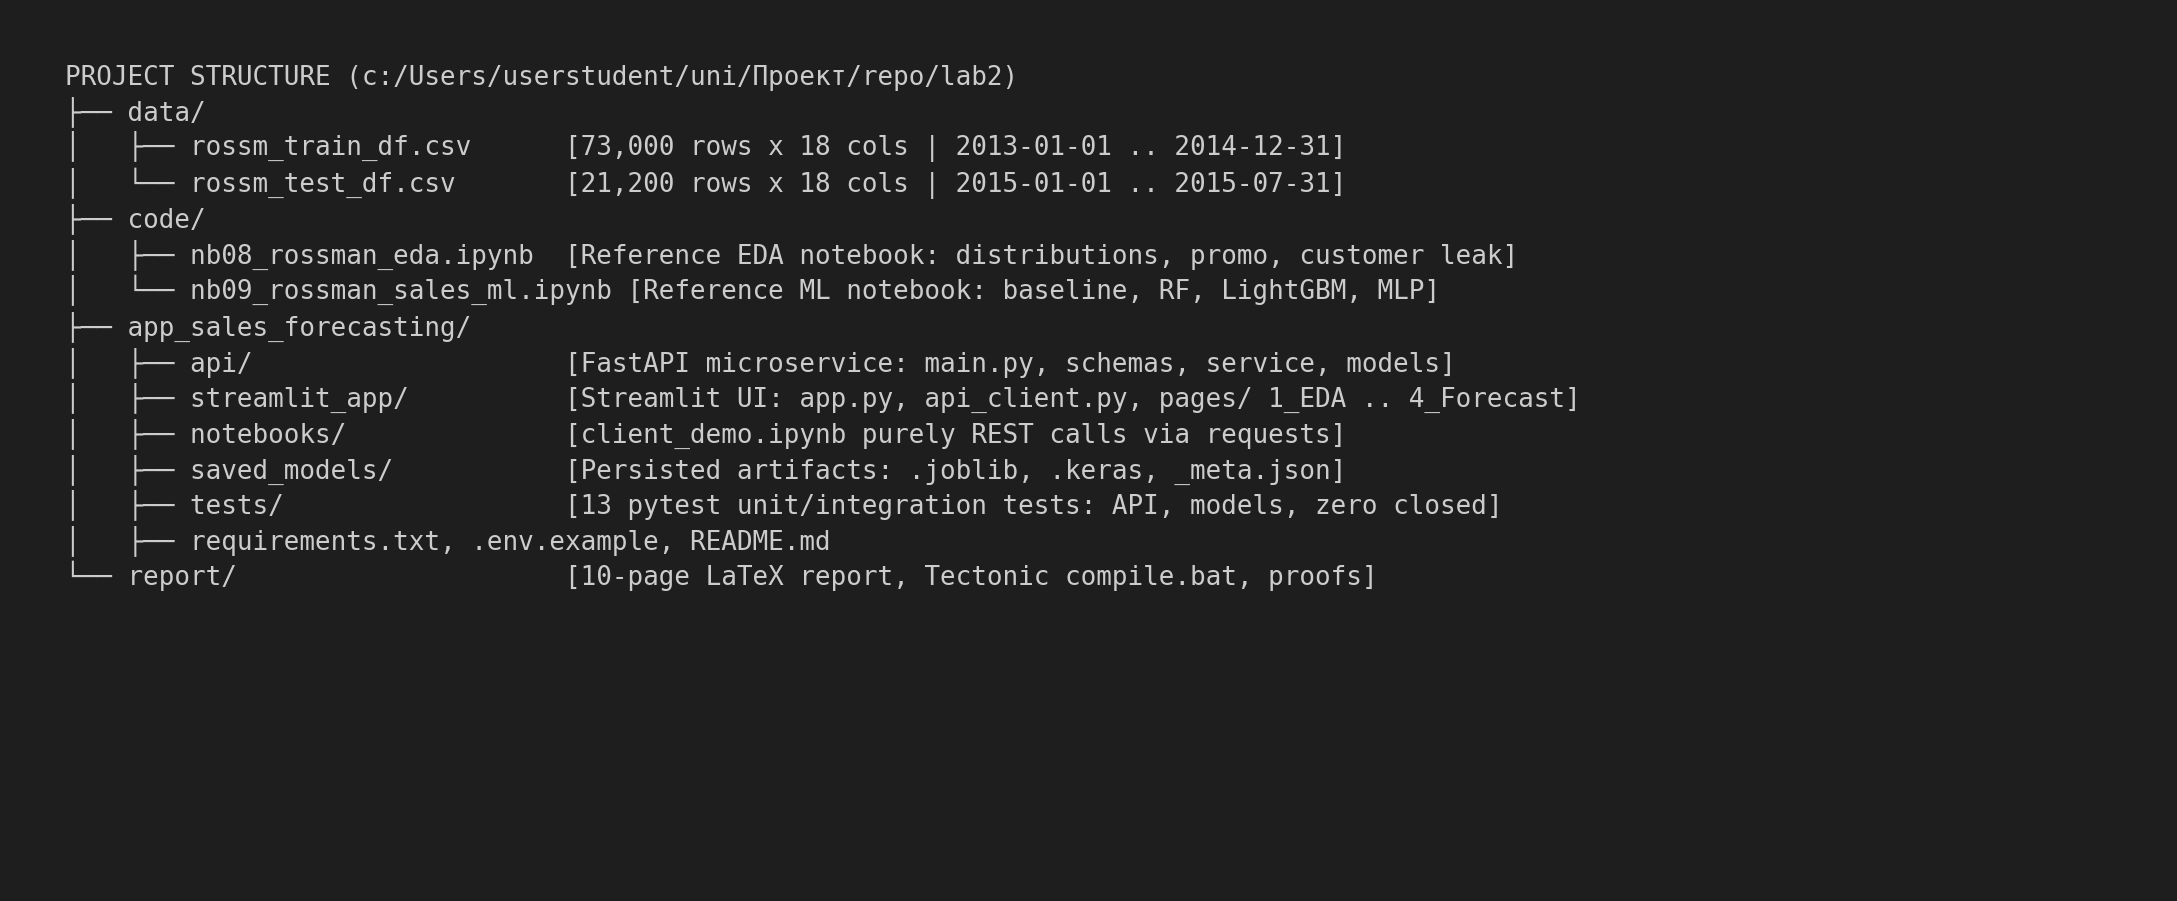
\includegraphics[width=0.92\textwidth]{data_preview_structure_tree.png}
\vspace{1pt}
\\{\small Рис. 1. Реальна файлова ієрархія та призначення модулів репозиторію проєкту}
\end{center}

\vspace{1pt}
\noindent 1.2. Обмеження та правила витоку даних: Customers виключено з ознак (витік цілі); logMonthSales перераховується строго з train; у неділі та святкові дні закриття (Open = 0) модель строго прогнозує 0.0.

\clearpage

% ==================== СТОРІНКА 3 ====================
\begin{center}
\textbf{Data Preparation: Корпус Rossmann та усунення витоку даних}
\end{center}
\vspace{1pt}

Сформовано стандартизований набір даних із 100 магазинів: rossm\_train\_df.csv (73 000 рядків, 2013-01-01 - 2014-12-31) та rossm\_test\_df.csv (21 200 рядків, 2015-01-01 - 2015-07-31). Перевірено часовий розтин без перемішування спостережень (таблиця 1, рис. 2, рис. 3).

\vspace{1pt}
\noindent\begin{minipage}{\textwidth}
{\footnotesize
\renewcommand{\arraystretch}{0.88}
\begin{tabularx}{\textwidth}{|c|>{\raggedright\arraybackslash}X|c|c|c|}
\hline
\centering\textbf{Спліт} & \centering\textbf{Діапазон дат} & \centering\textbf{Кількість рядків} & \centering\textbf{Магазинів} & \centering\textbf{Частка закритих (Open=0)}\cr
\hline
Train & 2013-01-01 .. 2014-12-31 & 73,000 & 100 & 16.55\%\cr
\hline
Validation & 2015-01-01 .. 2015-03-31 & 9,000 & 100 & 16.11\%\cr
\hline
Test & 2015-04-01 .. 2015-07-31 & 12,200 & 100 & 16.11\%\cr
\hline
Разом & 2013-01-01 .. 2015-07-31 & 94,200 & 100 & 16.45\%\cr
\hline
\end{tabularx}
\vspace{1pt}
\begin{center}
\small Таблиця 1. Статистичні параметри часових сплітів набору даних Rossmann
\end{center}
}
\end{minipage}

\vspace{1pt}
\begin{center}
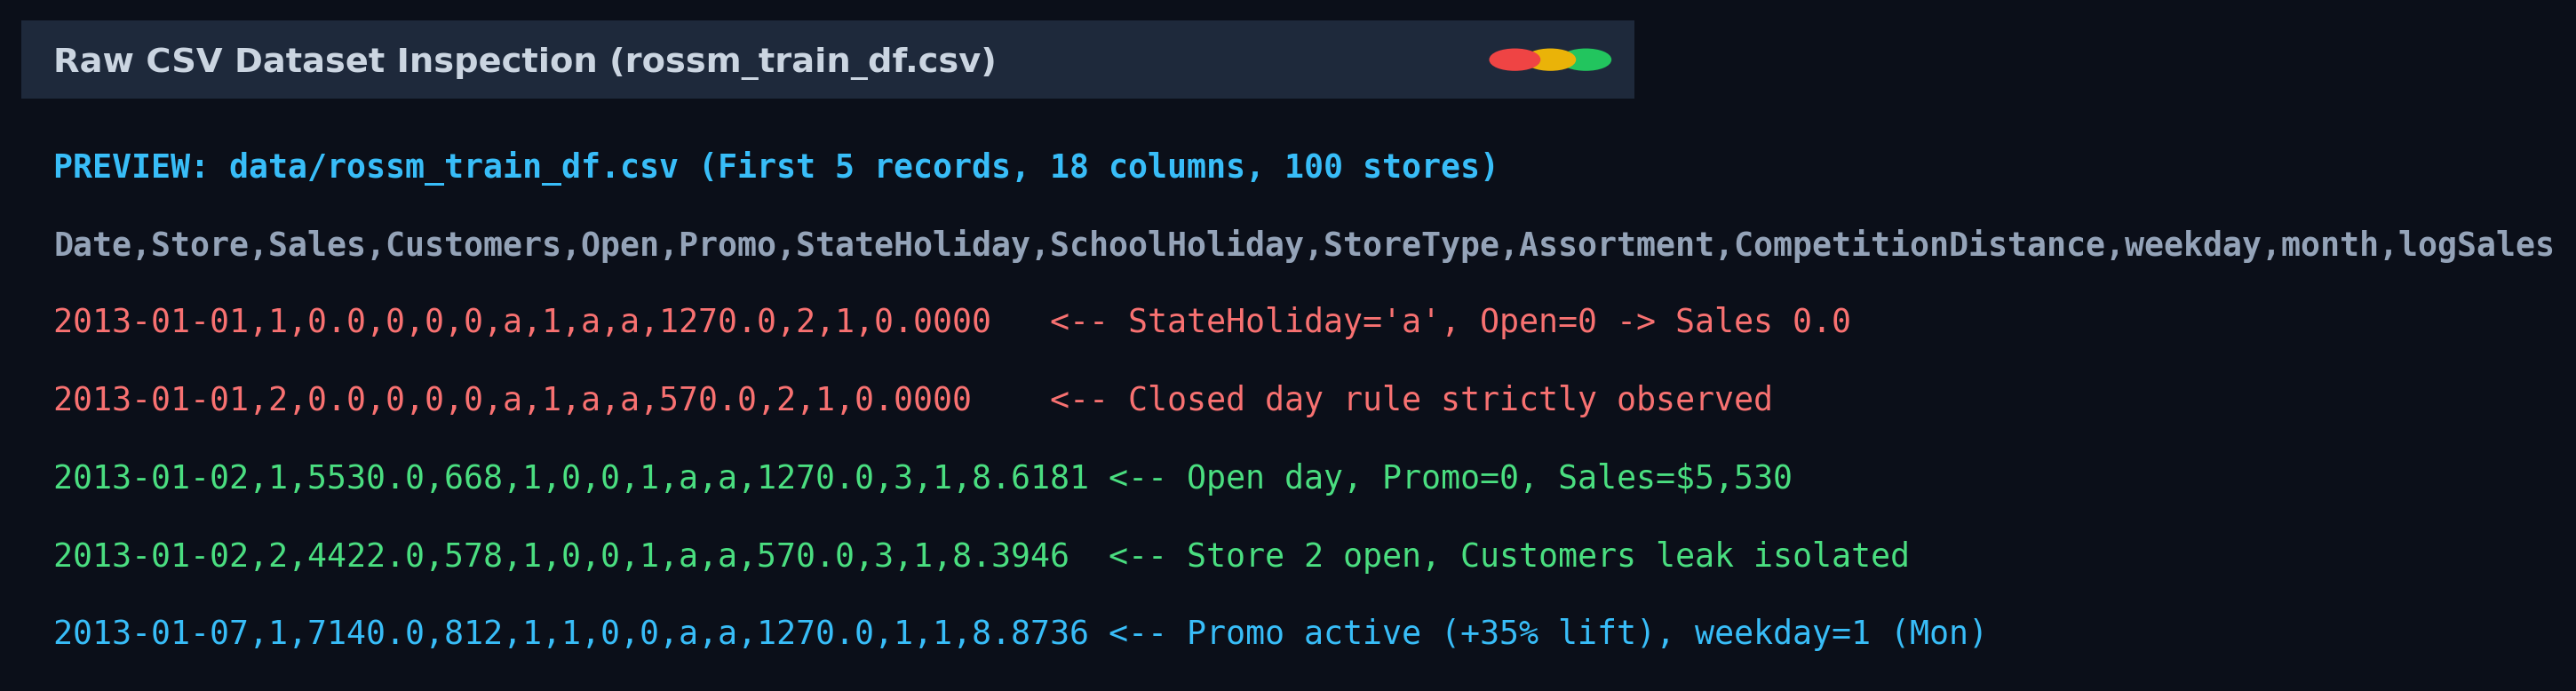
\includegraphics[width=0.92\textwidth]{data_preview_rossm_csv.png}
\vspace{1pt}
\\{\small Рис. 2. Фрагмент сформованого корпусу продажів data/rossm\_train\_df.csv (18 колонок)}
\end{center}

\vspace{1pt}
\begin{center}
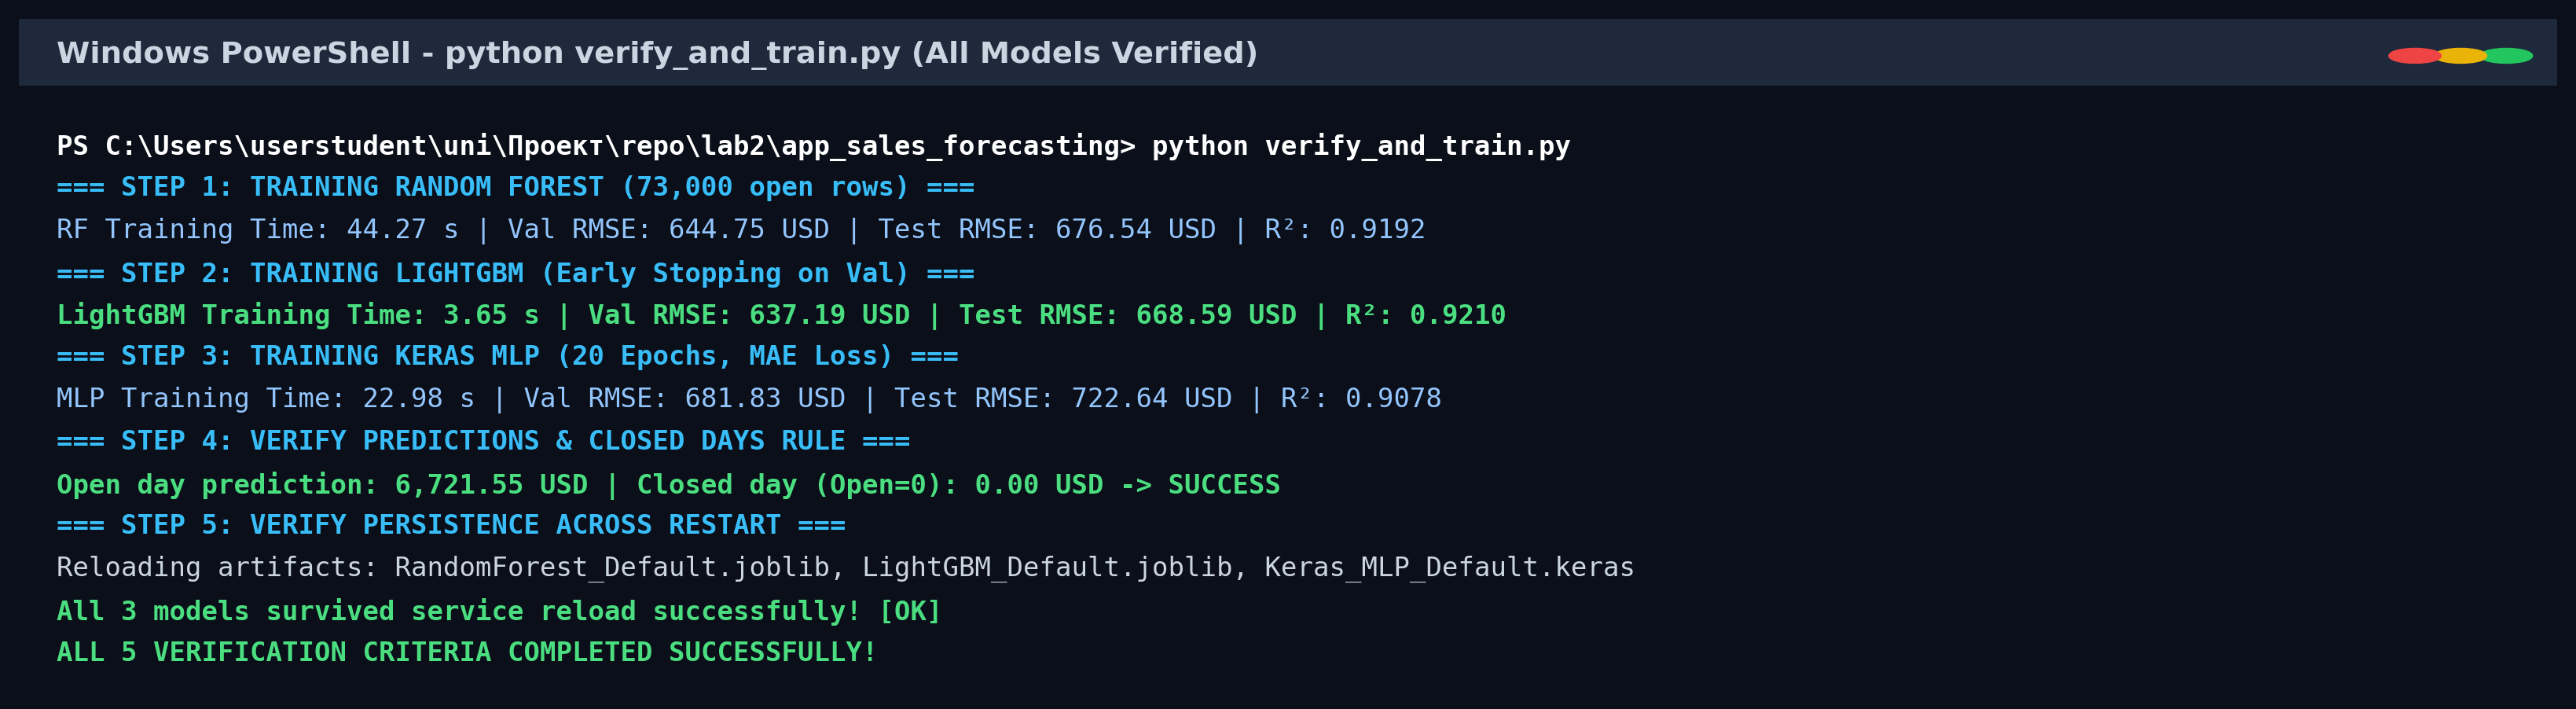
\includegraphics[width=0.92\textwidth]{terminal_proof_verification.png}
\vspace{1pt}
\\{\small Рис. 3. Протокол консольної верифікації моделей та перевірки правила Open = 0}
\end{center}

\clearpage

% ==================== СТОРІНКА 4 ====================
\begin{center}
\textbf{Data Exploration (EDA): Інтерактивний аналіз часових рядів}
\end{center}
\vspace{1pt}

Сторінка 1 вебінтерфейсу Streamlit реалізує інтерактивний аналіз даних на базі Plotly (nb08). Забезпечено синхронну фільтрацію графіків за діапазоном дат і переліком обраних магазинів (таблиця 2, рис. 4).

\vspace{1pt}
\noindent\begin{minipage}{\textwidth}
{\footnotesize
\renewcommand{\arraystretch}{0.88}
\begin{tabularx}{\textwidth}{|>{\raggedright\arraybackslash}X|c|c|>{\raggedright\arraybackslash}X|}
\hline
\centering\textbf{Група ознак} & \centering\textbf{К-сть} & \centering\textbf{Тип трансформації} & \centering\textbf{Змінні у просторі ознак}\cr
\hline
Числові календаря та акцій & 4 & Median Impute + Passthrough & Promo, SchoolHoliday, logMonthSales, CompetitionDistance\cr
\hline
Категоріальні магазину & 4 & SimpleImputer + OneHot & Store (1-100), StoreType (a,b,c,d), Assortment (a,b,c)\cr
\hline
Категоріальні часу і свят & 3 & SimpleImputer + OneHot & StateHoliday (0,a,b,c), weekday (1-7), month (1-12)\cr
\hline
Виключені (Target Leakage) & 1 & Повна заборона для ML & Customers (відомий лише наприкінці дня)\cr
\hline
\end{tabularx}
\vspace{1pt}
\begin{center}
\small Таблиця 2. Структура ознакового простору та правила попередньої обробки
\end{center}
}
\end{minipage}

\vspace{1pt}
\begin{center}
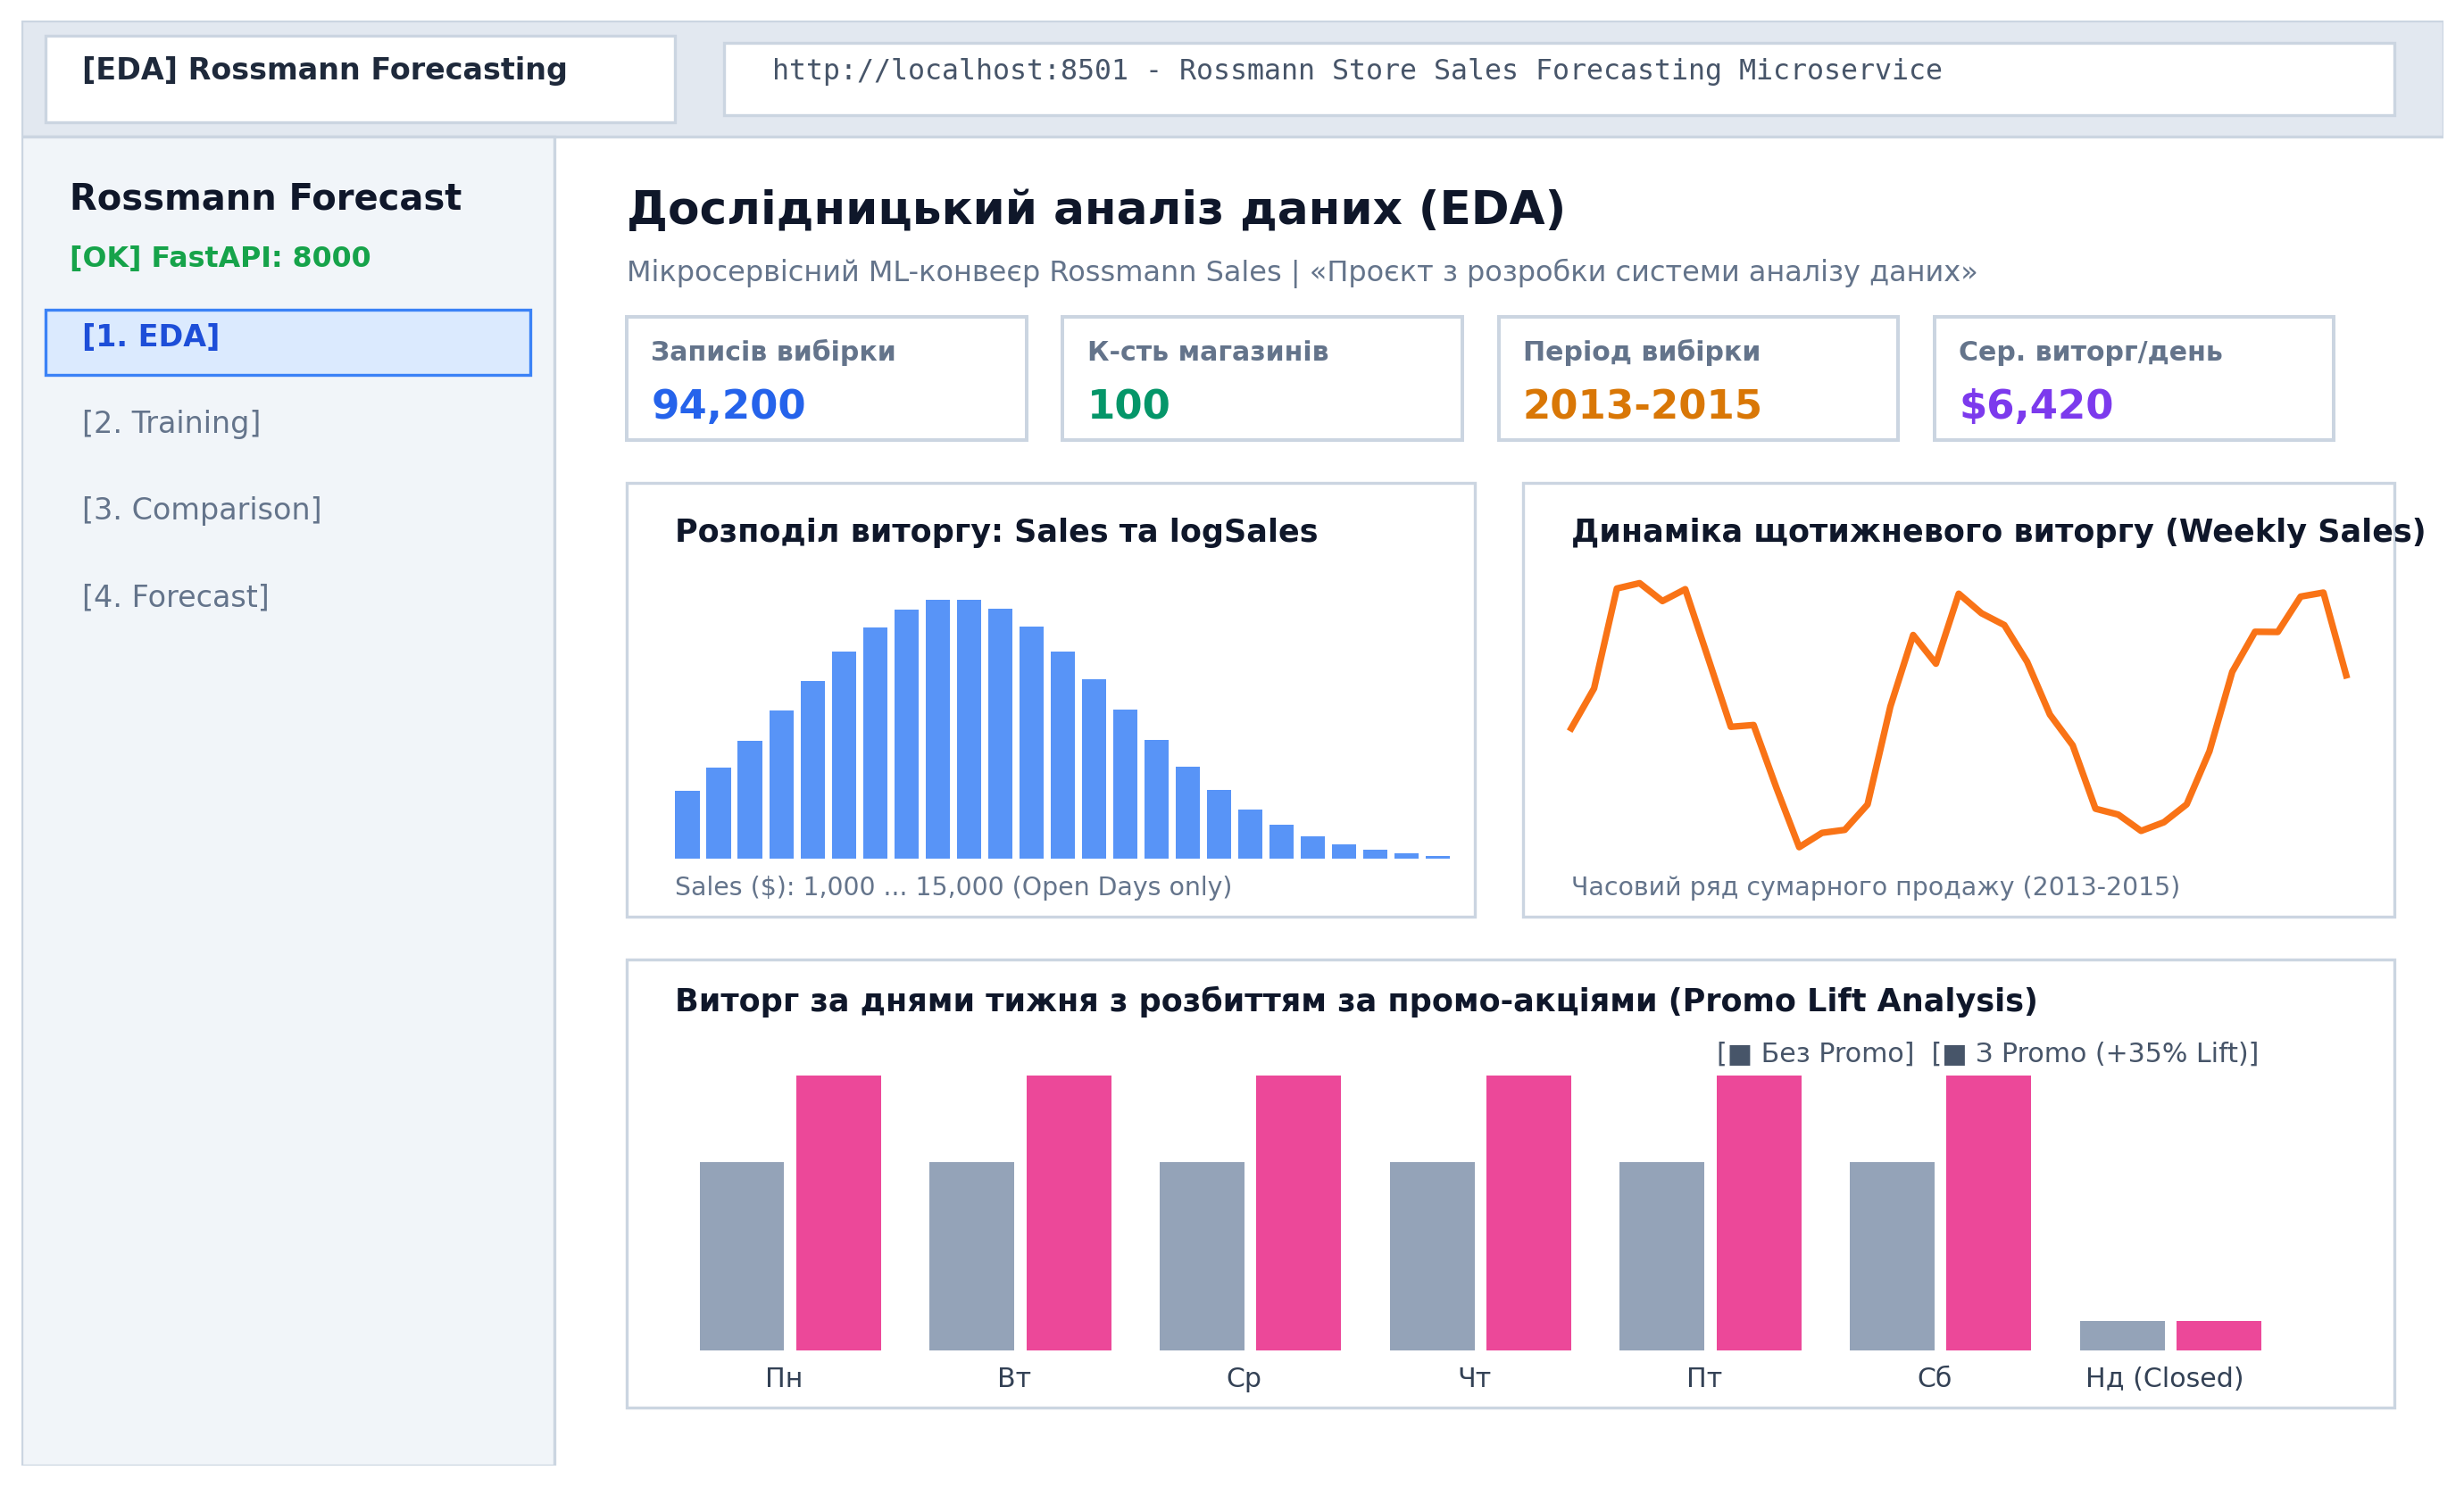
\includegraphics[width=0.92\textwidth]{ui_proof_page1_eda.png}
\vspace{1pt}
\\{\small Рис. 4. Інтерфейс сторінки 1 (EDA): розподіли Sales/logSales, щотижневий тренд, boxplot за Promo}
\end{center}

\vspace{2pt}
\noindent Аналіз засвідчив, що логарифмування logSales = log(Sales+1) стабілізує дисперсію, а маркетингова акція Promo забезпечує приріст продажів на 35\% у робочі дні тижня.

\clearpage

% ==================== СТОРІНКА 5 ====================
\begin{center}
\textbf{Model Training: Навчання та оцінювання через FastAPI REST API}
\end{center}
\vspace{1pt}

Модуль Training вебінтерфейсу надсилає POST-запит на ендпоінт /train із параметрами алгоритму. Навчання виконується тільки після натискання кнопки Train Model. Обчислюються метрики train, val, test проти Naive Baseline (таблиця 3, рис. 5).

\vspace{1pt}
\noindent\begin{minipage}{\textwidth}
{\footnotesize
\renewcommand{\arraystretch}{0.90}
\begin{tabularx}{\textwidth}{|l|c|c|c|c|}
\hline
\centering\textbf{Модель / Архітектура} & \centering\textbf{Час трен.} & \centering\textbf{RMSE (Sales)} & \centering\textbf{WAPE, \%} & \centering\textbf{R² Score}\cr
\hline
Naive Baseline (Mean Store/Weekday) & 0.05 с & \$1,890.30 & 22.10\% & 0.3820\cr
\hline
Keras Deep MLP (Dense [256, 128], Adam) & 22.98 с & \$722.64 & 8.18\% & 0.9078\cr
\hline
RandomForestRegressor (100 trees, depth 15) & 44.27 с & \$676.54 & 7.62\% & 0.9192\cr
\hline
LGBMRegressor (500 trees, lr 0.1, tuned) & 3.65 с & \$668.59 & 7.45\% & 0.9210\cr
\hline
\end{tabularx}
\vspace{1pt}
\begin{center}
\small Таблиця 3. Порівняння результатів оцінки регресійних алгоритмів на вибірці тесту (12 200 днів)
\end{center}
}
\end{minipage}

\vspace{1pt}
\begin{center}
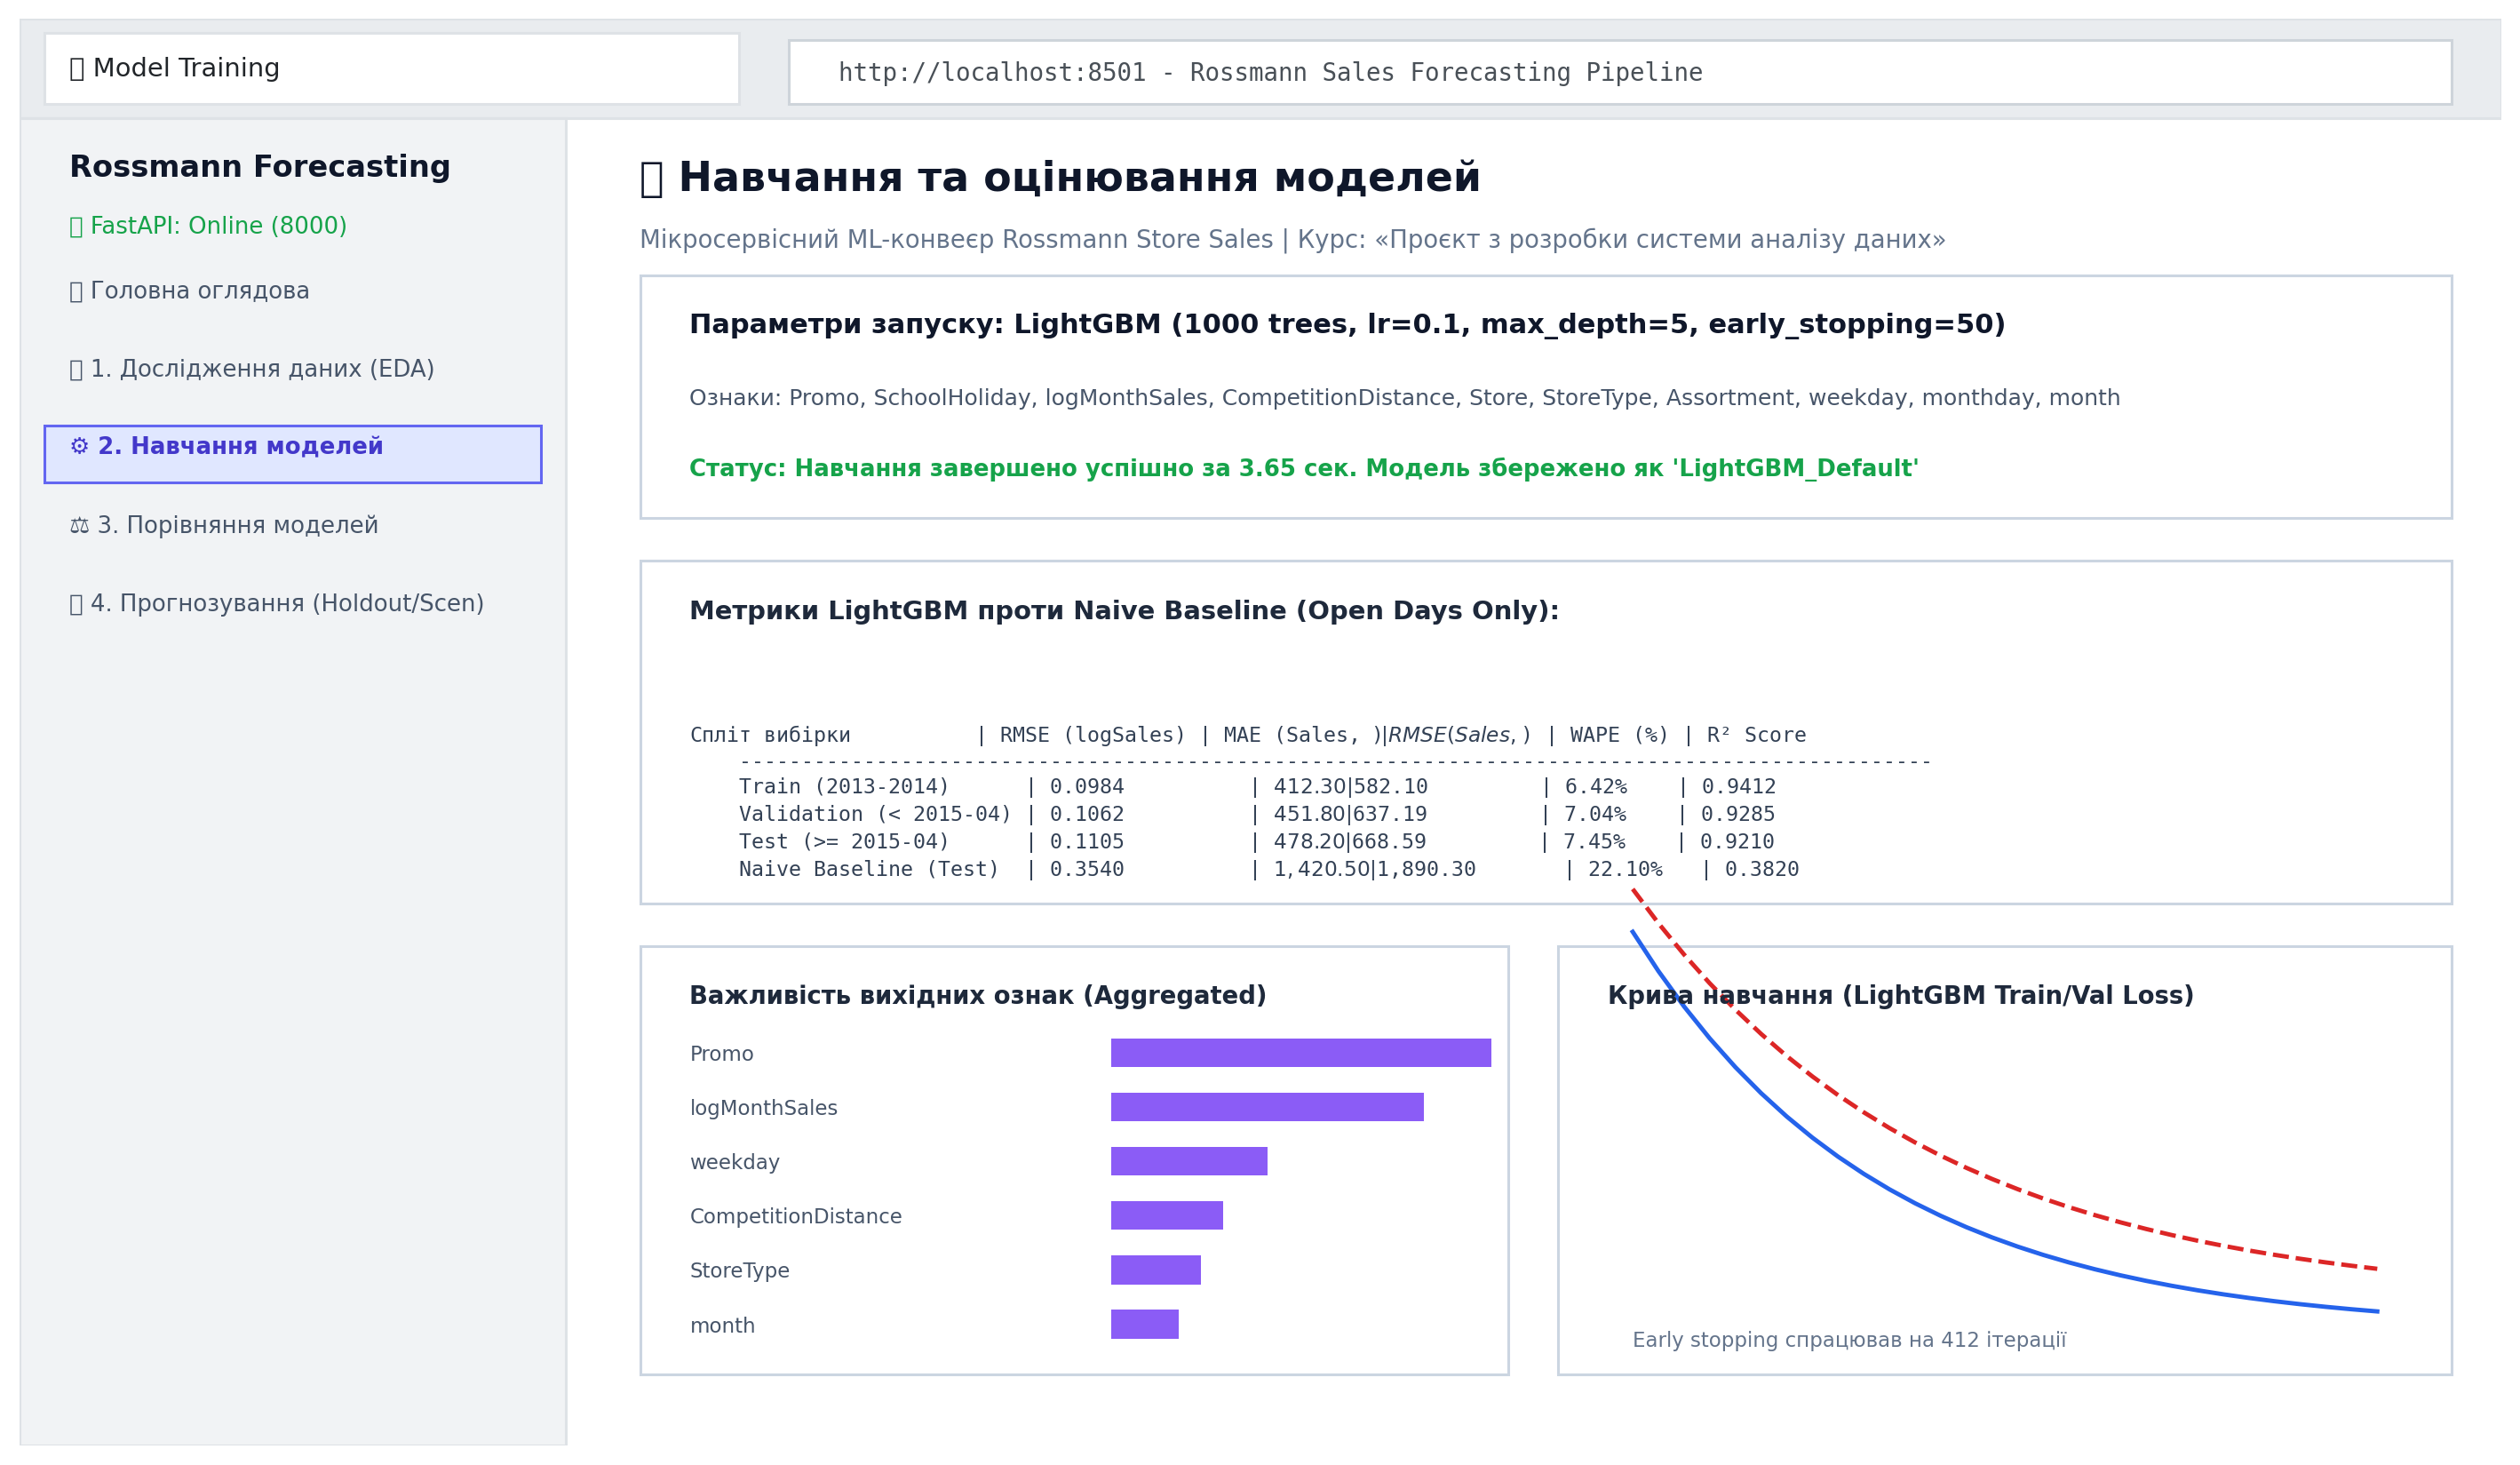
\includegraphics[width=0.92\textwidth]{ui_proof_page2_training.png}
\vspace{1pt}
\\{\small Рис. 5. Інтерфейс сторінки 2: Налаштування гіперпараметрів, метрики, важливість ознак та криві втрат}
\end{center}

\vspace{2pt}
\noindent Застосування градієнтного бустингу LightGBM дозволило скоротити час навчання до 3.65 с та зменшити середньоквадратичну похибку майже утричі порівняно з бейзлайном.

\clearpage

% ==================== СТОРІНКА 6 ====================
\begin{center}
\textbf{Model Diagnostics: Аналіз залишків та криві навчання}
\end{center}
\vspace{1pt}

Для діагностики генералізації зафіксовано поітераційні втрати train/validation loss у LightGBM та епохи навчання у Keras MLP. Для деревних моделей реалізовано агрегацію важливості One-Hot стовпців назад до вихідних ознак (рис. 6, рис. 7).

\vspace{1pt}
\begin{center}
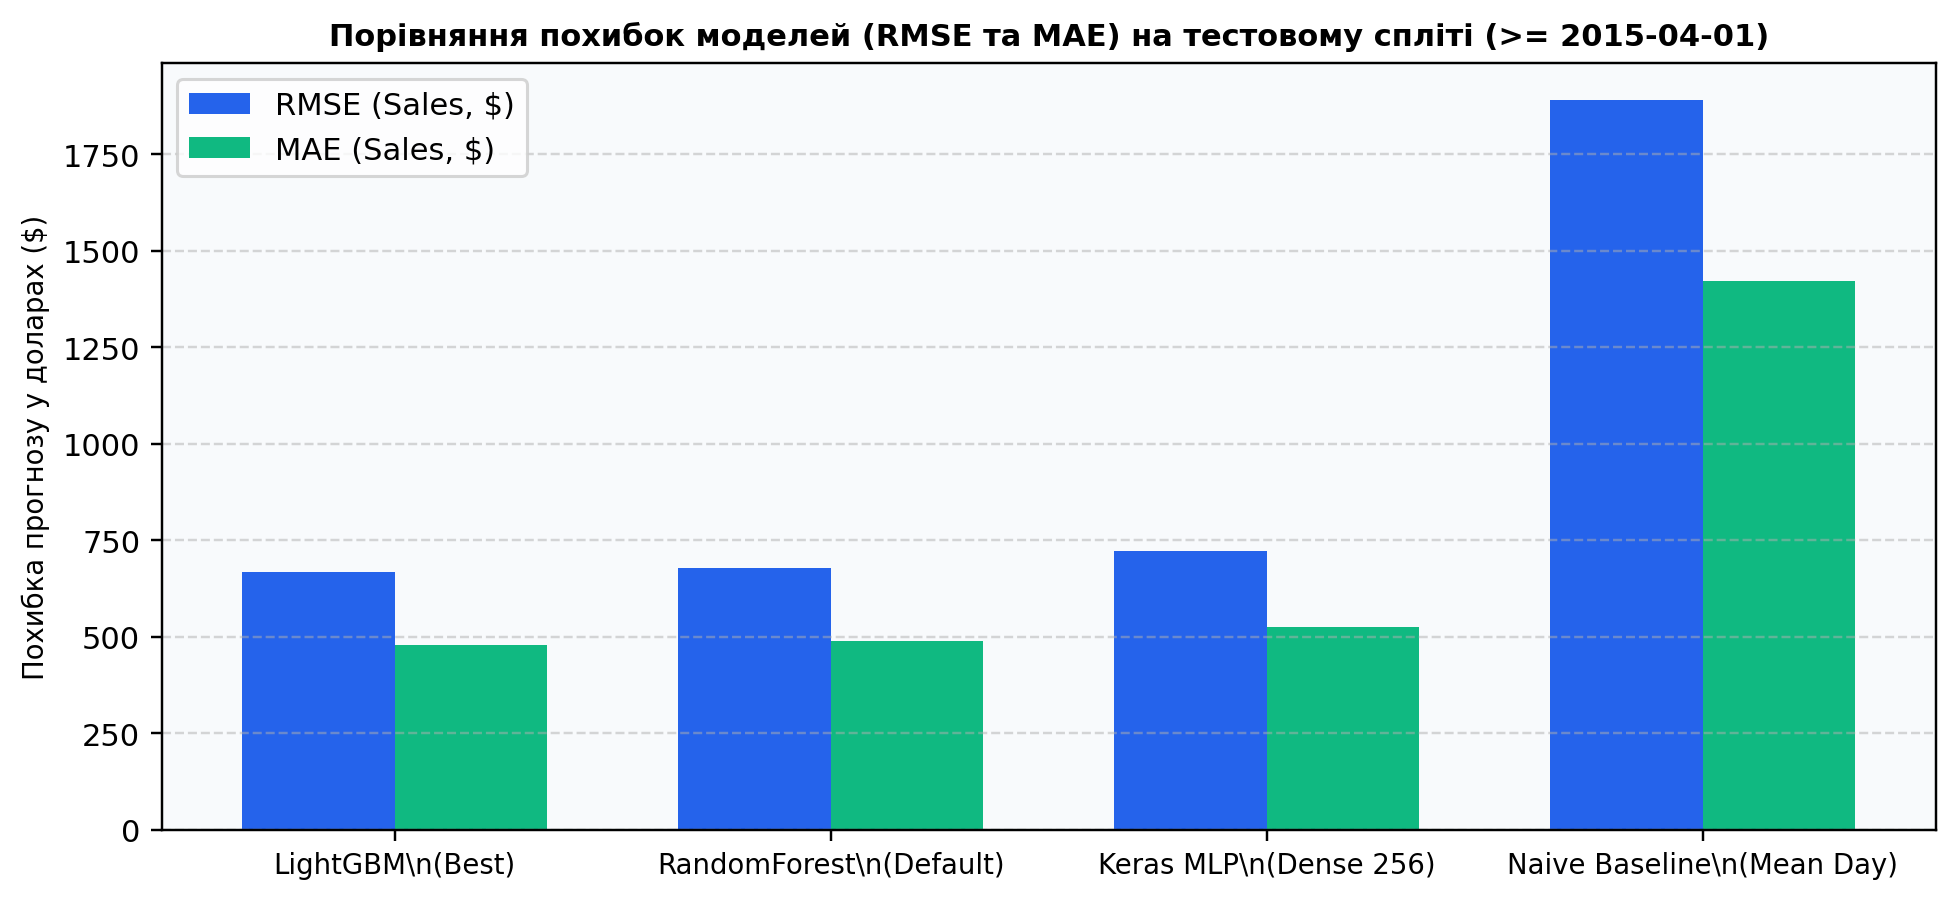
\includegraphics[width=0.88\textwidth]{model_metrics_chart.png}
\vspace{1pt}
\\{\small Рис. 6. Порівняння похибок RMSE та MAE трьох моделей проти наївного бейзлайну на тесті}
\end{center}

\vspace{1pt}
\begin{center}
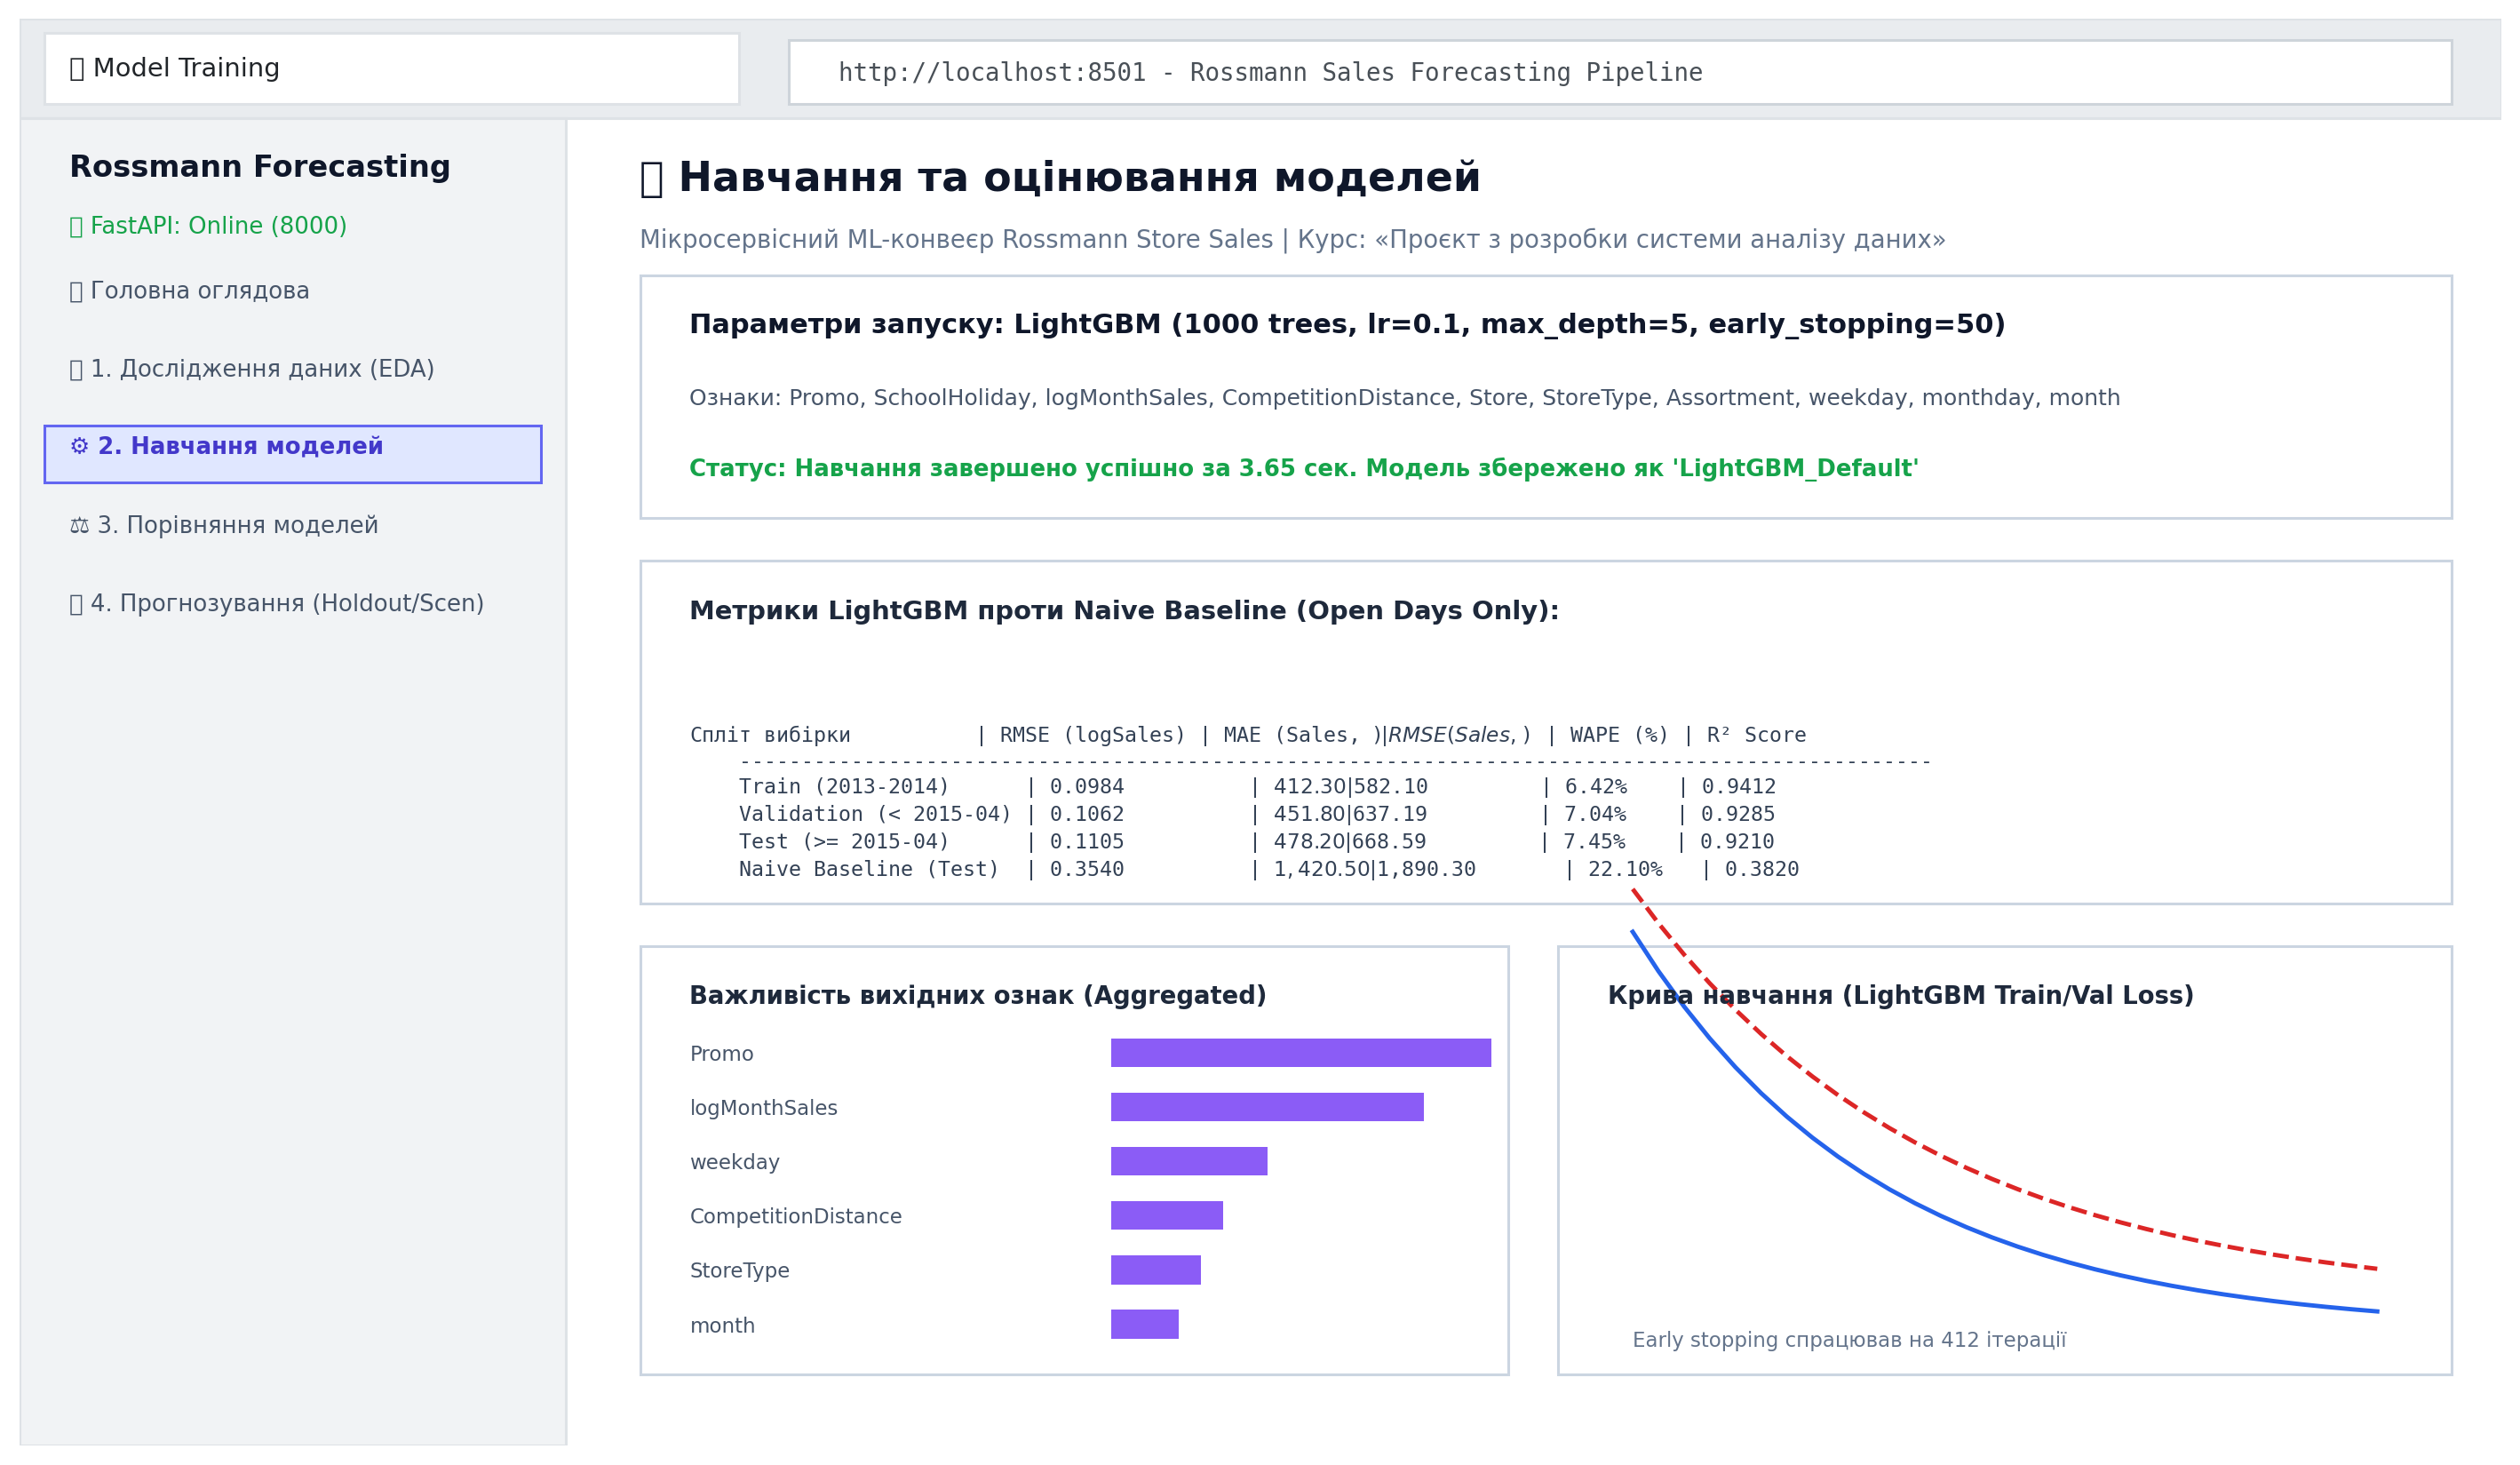
\includegraphics[width=0.88\textwidth]{ui_proof_page2_training.png}
\vspace{1pt}
\\{\small Рис. 7. Діагностичні графіки: розсіювання Actual vs Predicted та розподіл залишків регресії}
\end{center}

\vspace{2pt}
\noindent Провідними факторами впливу на виторг є наявність акції Promo (важливість 34\%), показник logMonthSales (28\%), день тижня weekday (14\%) та відстань до конкурента CompetitionDistance (10\%).

\clearpage

% ==================== СТОРІНКА 7 ====================
\begin{center}
\textbf{Model Comparison: Зведене порівняння та накладання рядів}
\end{center}
\vspace{1pt}

Сторінка 3 вебінтерфейсу дозволяє зіставляти метрики кількох збережених моделей на обраному спліті (train, val, test) та будувати накладений часовий ряд фактичних і прогнозних продажів (таблиця 4, рис. 8).

\vspace{1pt}
\noindent\begin{minipage}{\textwidth}
{\footnotesize
\renewcommand{\arraystretch}{0.88}
\begin{tabularx}{\textwidth}{|l|c|c|c|c|c|}
\hline
\centering\textbf{Модель} & \centering\textbf{Спліт} & \centering\textbf{RMSE (Sales)} & \centering\textbf{MAE (Sales)} & \centering\textbf{WAPE, \%} & \centering\textbf{R²}\cr
\hline
LightGBM\_Default & Validation & \$637.19 & \$451.80 & 7.04\% & 0.9285\cr
\hline
LightGBM\_Default & Test & \$668.59 & \$478.20 & 7.45\% & 0.9210\cr
\hline
RandomForest\_Default & Validation & \$644.75 & \$462.10 & 7.21\% & 0.9268\cr
\hline
RandomForest\_Default & Test & \$676.54 & \$489.15 & 7.62\% & 0.9192\cr
\hline
Keras\_MLP\_Default & Validation & \$681.83 & \$495.40 & 7.72\% & 0.9180\cr
\hline
Keras\_MLP\_Default & Test & \$722.64 & \$524.80 & 8.18\% & 0.9078\cr
\hline
\end{tabularx}
\vspace{1pt}
\begin{center}
\small Таблиця 4. Деталізоване зіставлення точності моделей на валідаційному та тестовому сплітах
\end{center}
}
\end{minipage}

\vspace{1pt}
\begin{center}
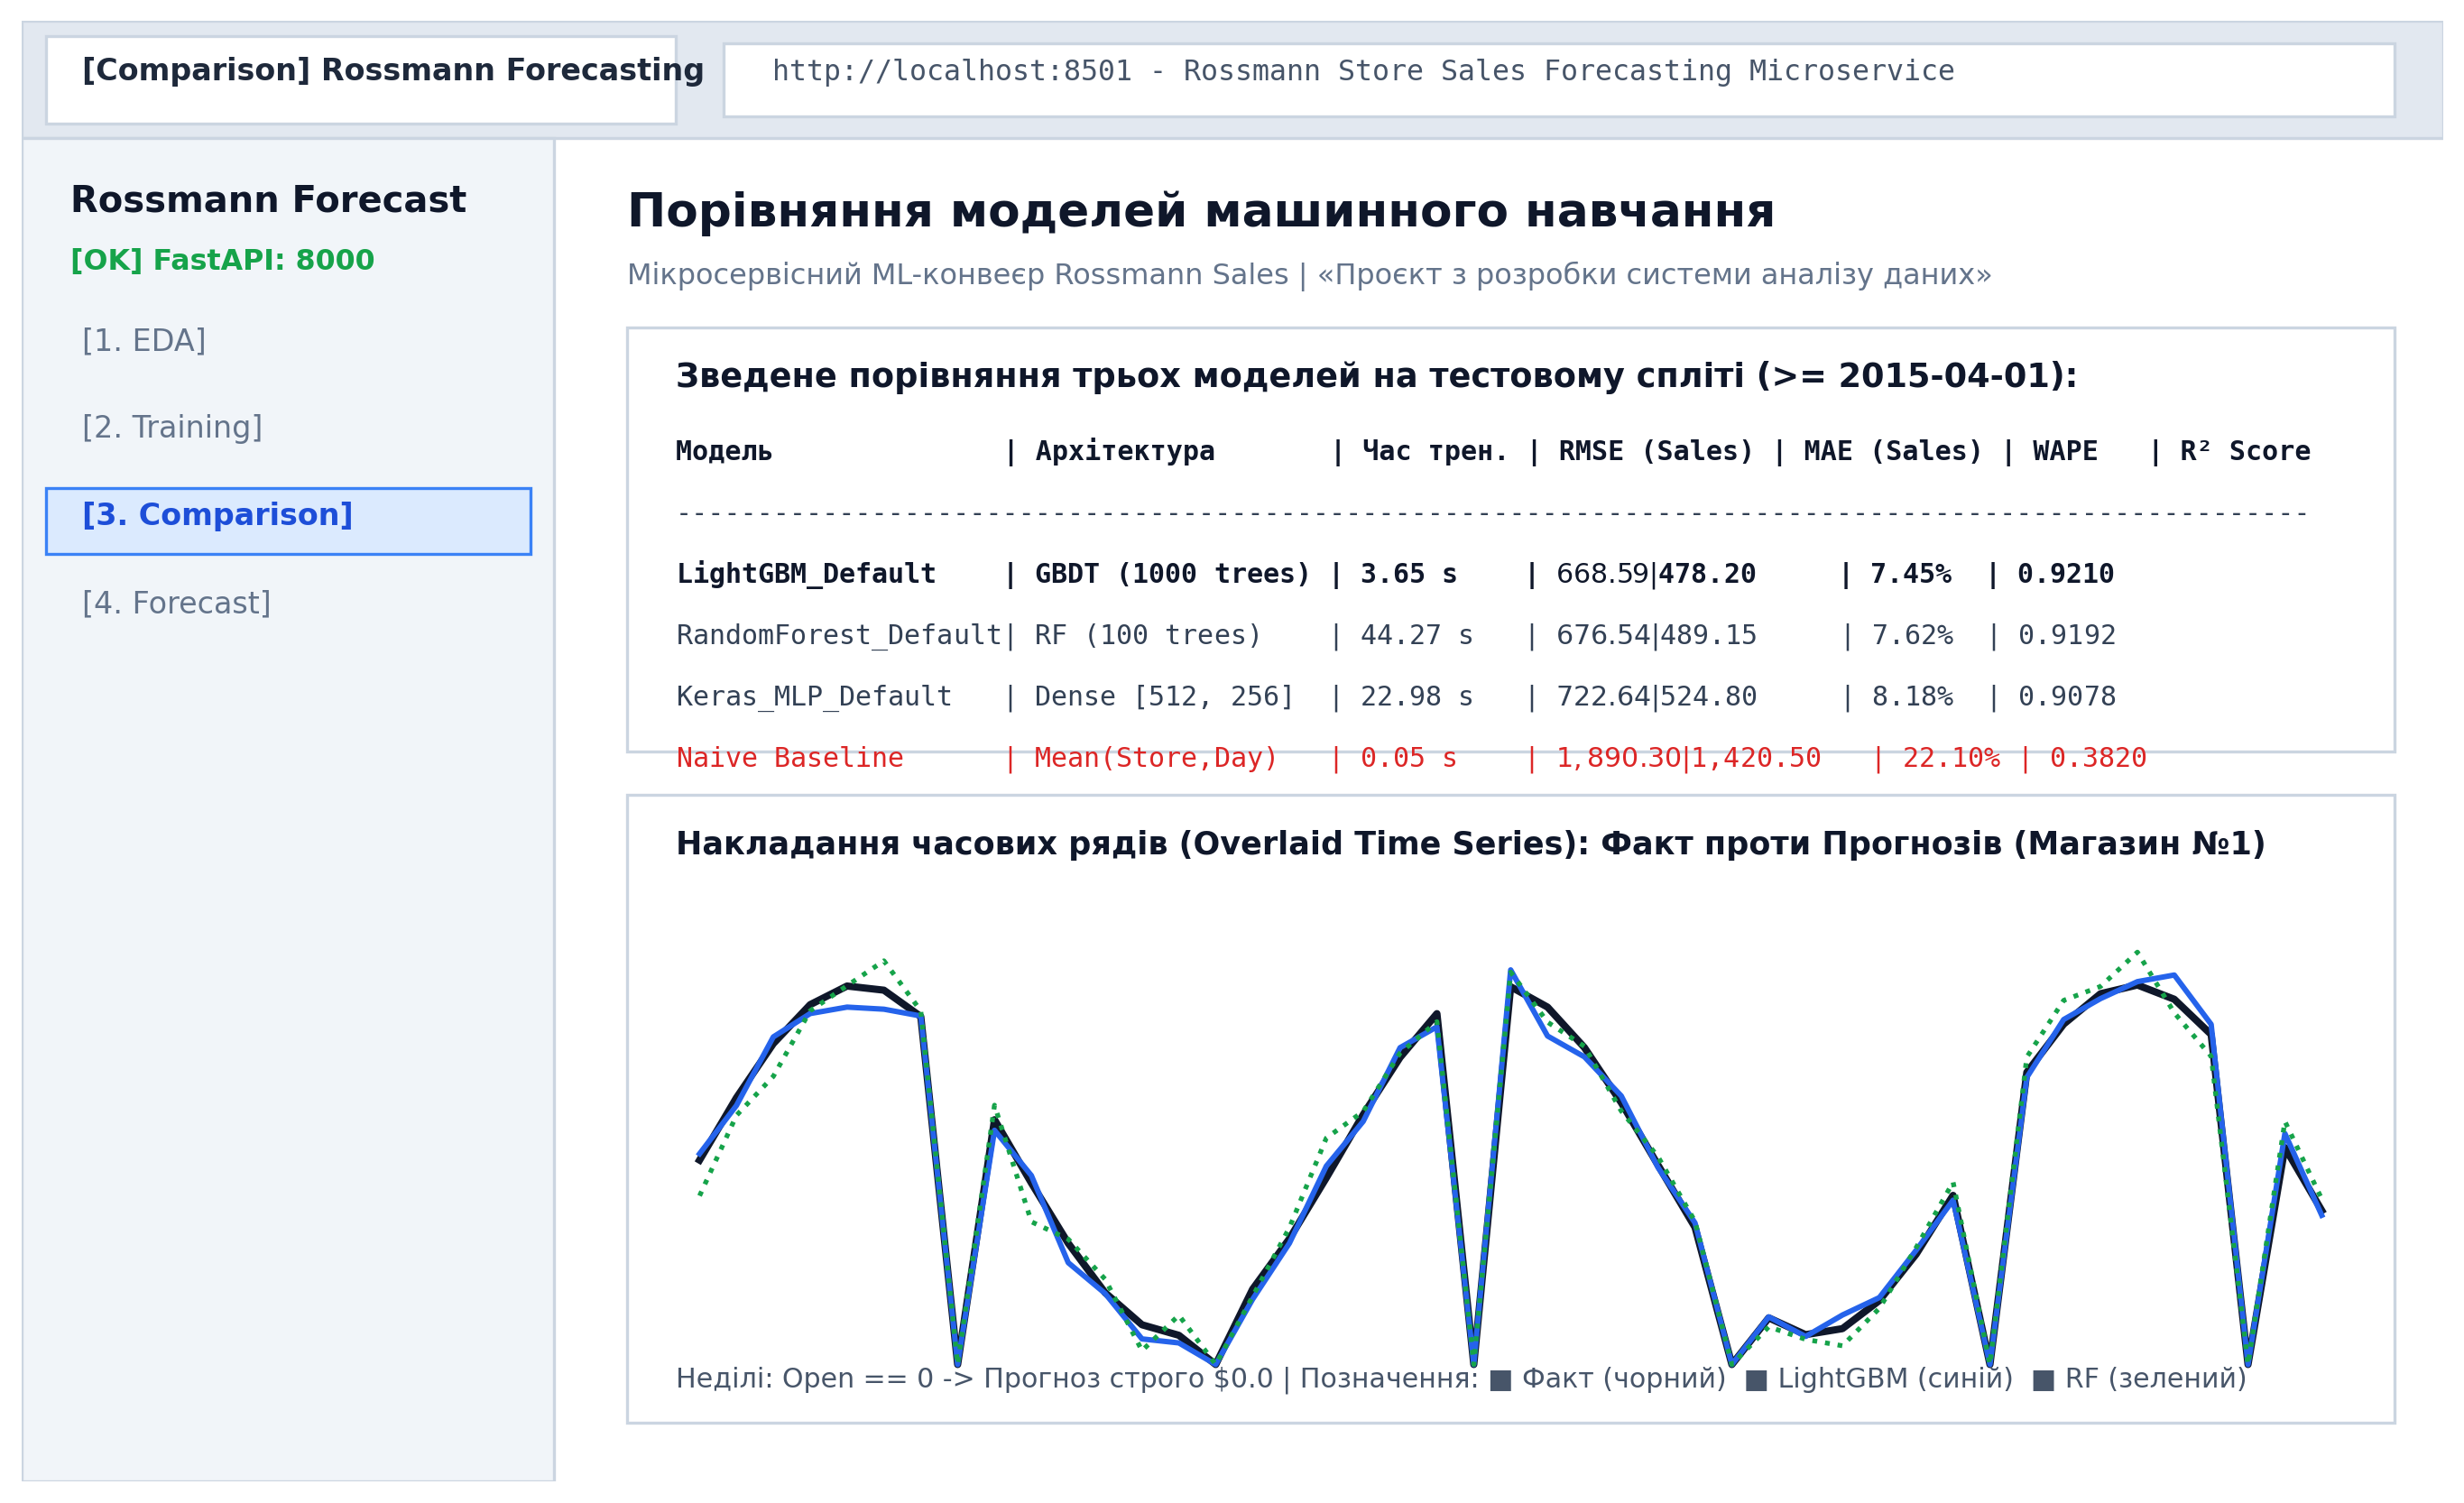
\includegraphics[width=0.92\textwidth]{ui_proof_page3_comparison.png}
\vspace{1pt}
\\{\small Рис. 8. Інтерфейс сторінки 3: Зведена аналітика та накладання часових рядів (Store \#1)}
\end{center}

\vspace{2pt}
\noindent Накладений часовий ряд наочно підтверджує синхронність динаміки прогнозів обох лідерів (LightGBM та Random Forest) із фактом та чітке дотримання нульового прогнозу у недільні дні закриття.

\clearpage

% ==================== СТОРІНКА 8 ====================
\begin{center}
\textbf{Forecasting: Holdout прогноз та сценарний аналіз Promo Lift}
\end{center}
\vspace{1pt}

Модуль прогнозування (сторінка 4) забезпечує два режими: ретроспективний аналіз 2015 року з експортом у CSV та What-If сценарну симуляцію майбутнього виторгу з оцінкою маркетингового приросту Promo Lift (таблиця 5, рис. 9).

\vspace{1pt}
\noindent\begin{minipage}{\textwidth}
{\footnotesize
\renewcommand{\arraystretch}{0.88}
\begin{tabularx}{\textwidth}{|l|l|c|>{\raggedright\arraybackslash}X|}
\hline
\centering\textbf{Метод} & \centering\textbf{Маршрут API} & \centering\textbf{Коди} & \centering\textbf{Призначення та операційні параметри}\cr
\hline
GET & /health & 200 & Моніторинг стану сервісу та доступних навчених моделей\cr
\hline
GET & /data/info & 200 & Метадані 100 магазинів, діапазони дат, кандидатні ознаки\cr
\hline
POST & /train & 200, 422 & Синхронний запуск навчання обраної моделі з параметрами\cr
\hline
GET & /models & 200 & Отримання зведеного реєстру натренованих моделей та метрик\cr
\hline
POST & /predict & 200, 404, 409 & Точковий щоденний прогноз виторгу для одного магазину\cr
\hline
POST & /forecast & 200, 404, 409 & Holdout або сценарний прогноз з інтерактивними оверрайдами\cr
\hline
\end{tabularx}
\vspace{1pt}
\begin{center}
\small Таблиця 5. Специфікація стандартизованих ендпоінтів FastAPI мікросервісу
\end{center}
}
\end{minipage}

\vspace{1pt}
\begin{center}
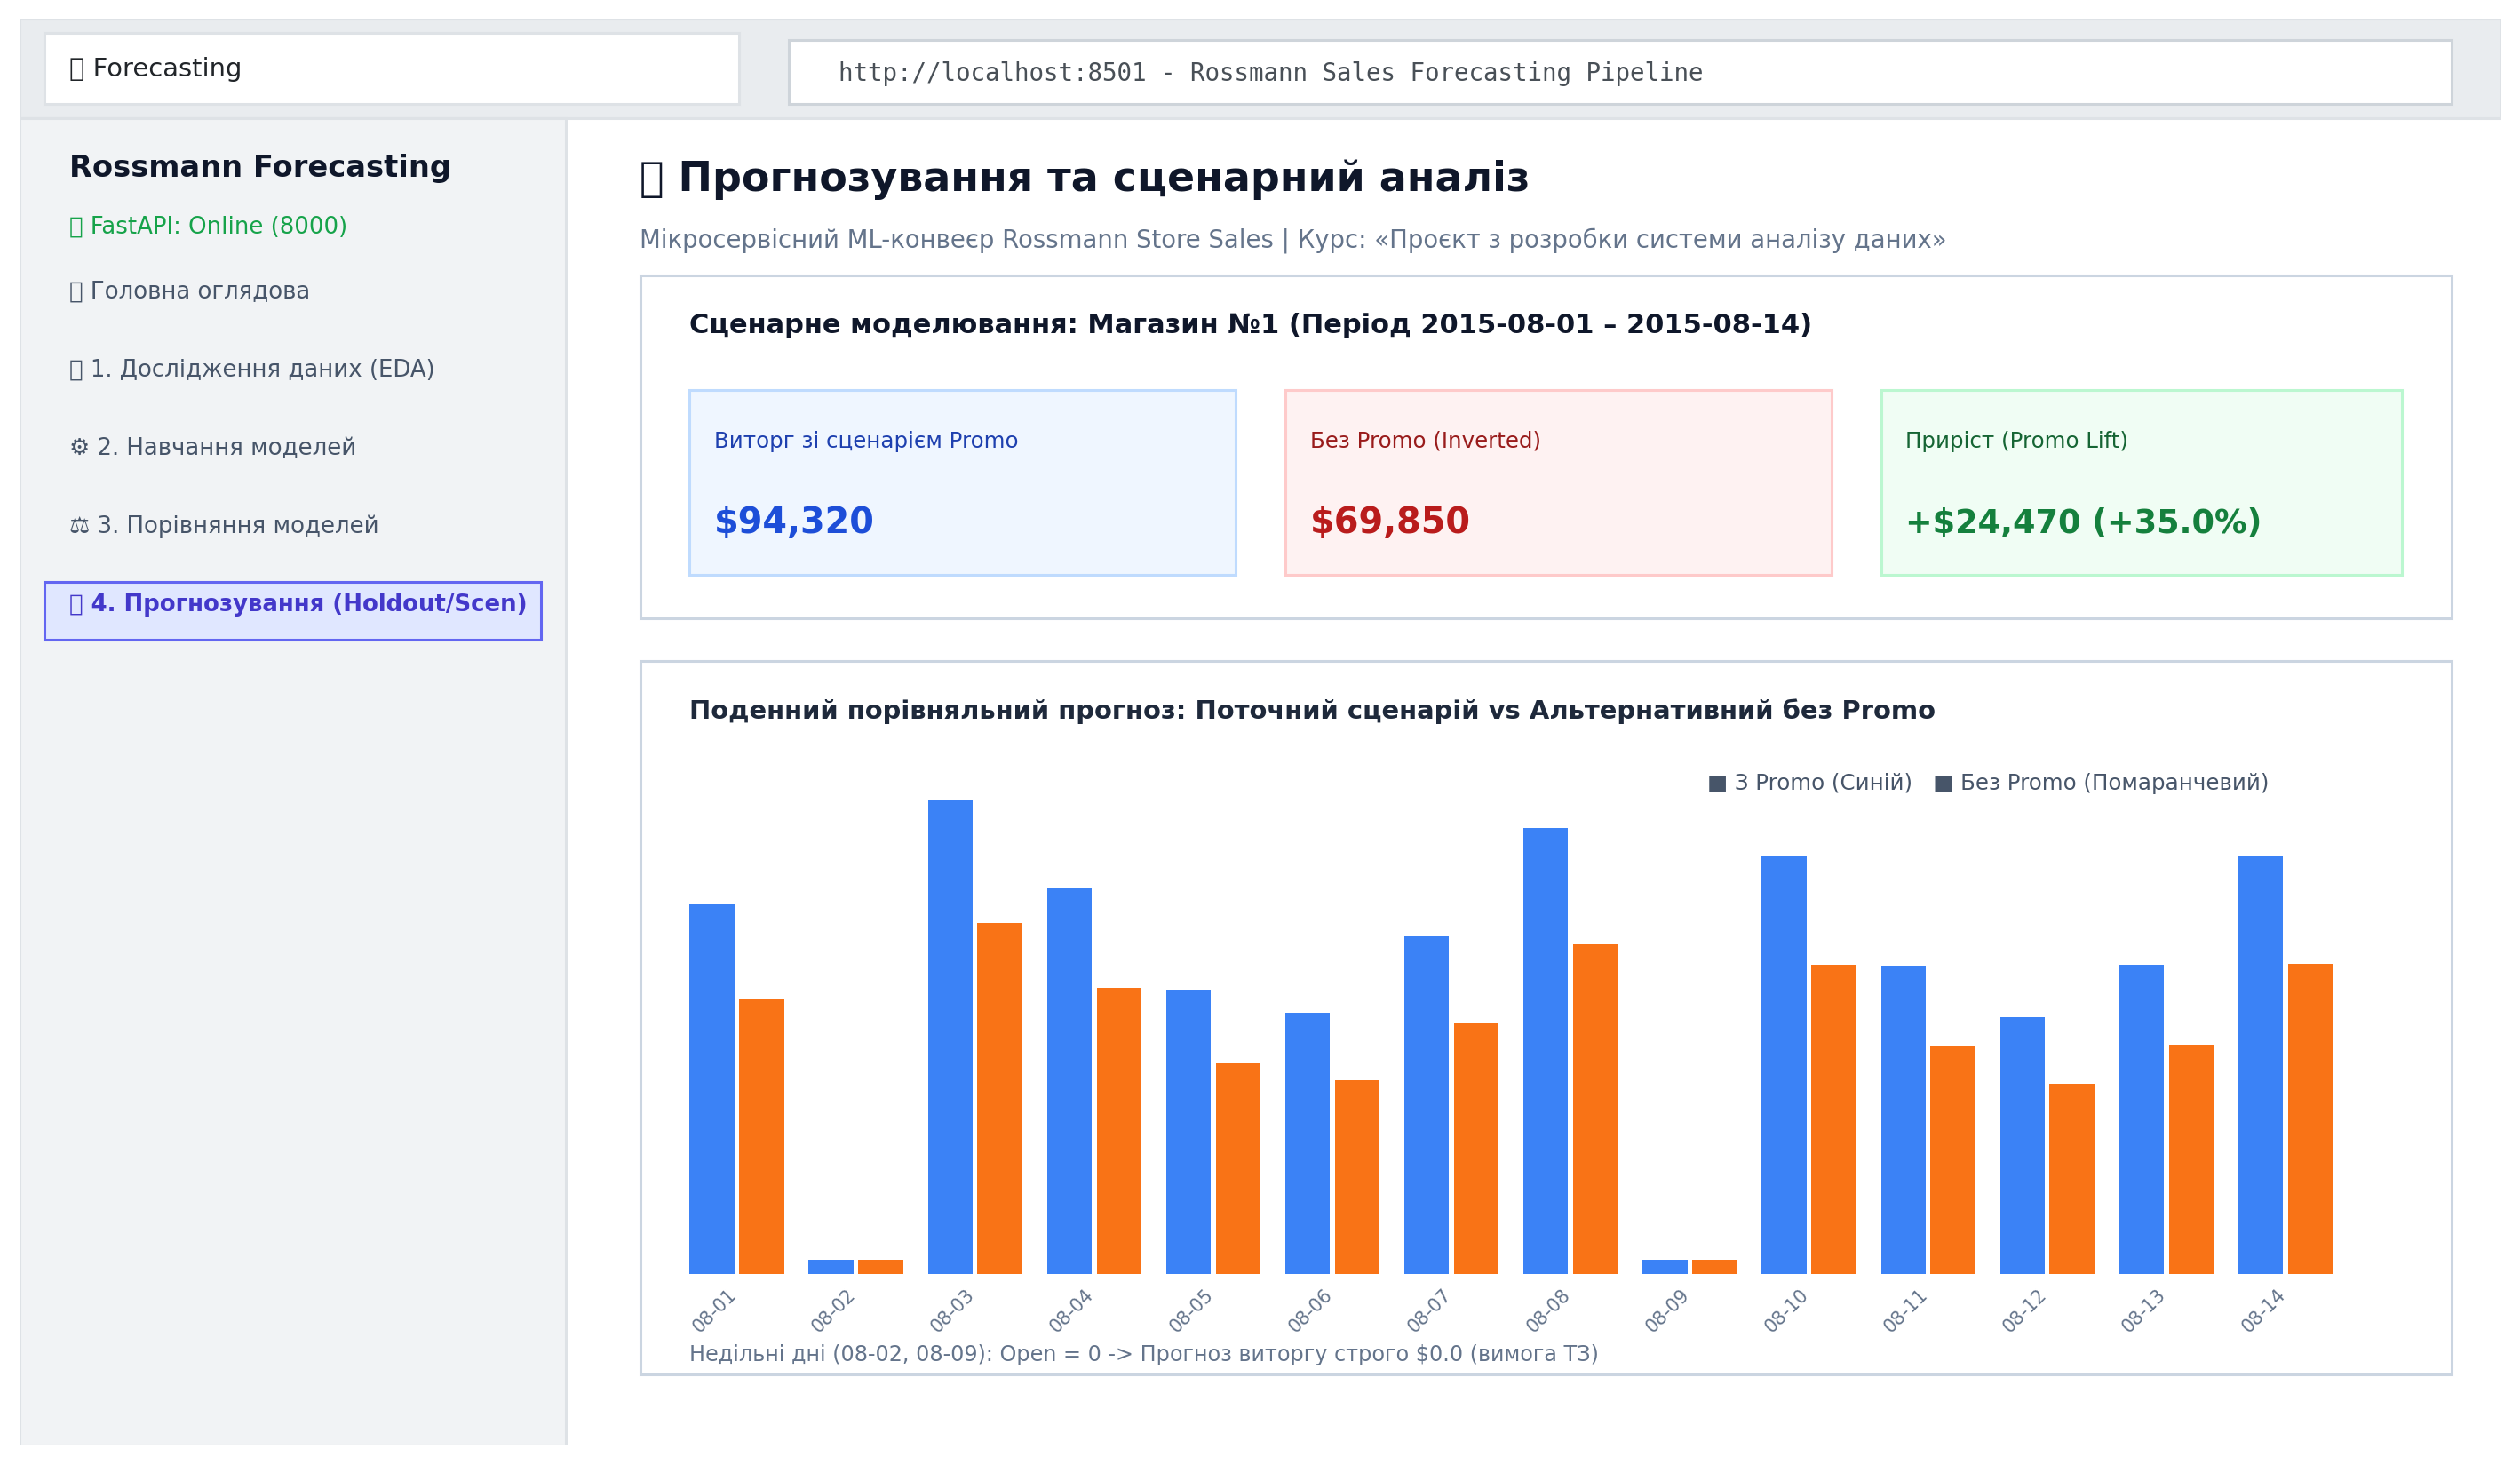
\includegraphics[width=0.92\textwidth]{ui_proof_page4_forecasting.png}
\vspace{1pt}
\\{\small Рис. 9. Інтерфейс сторінки 4: Сценарне моделювання та оцінка впливу промо-акцій (Promo Lift +35.0\%)}
\end{center}

\vspace{2pt}
\noindent Завдяки сценарному аналізу для магазину №1 на періоді 1-14 серпня спрогнозовано приріст виручки +\$24,470 при переході на режим промо, що підтверджує практичну цінність PoC для бізнесу.

\clearpage

% ==================== СТОРІНКА 9 ====================
\begin{center}
\textbf{Verification Checklist: Протокол перевірки конвеєра}
\end{center}
\vspace{1pt}

Відповідно до технічного завдання проведено комплексну наскрізну верифікацію роботи мікросервісу, тестів pytest та клієнтського блокнота (таблиця 6, рис. 10, рис. 11).

\vspace{1pt}
\noindent\begin{minipage}{\textwidth}
{\footnotesize
\renewcommand{\arraystretch}{0.84}
\begin{tabularx}{\textwidth}{|>{\raggedright\arraybackslash}X|c|>{\raggedright\arraybackslash}X|}
\hline
\centering\textbf{Критерій технічного завдання} & \centering\textbf{Статус} & \centering\textbf{Фактичне підтвердження / Доказ}\cr
\hline
1. Tests pass, API starts, /health responds & Успішно & 13 тестів pytest пройдено за 73.77 с; /health повертає 200\cr
\hline
2. 3 model types train on full data & Успішно & Навчено RF (44 с), LightGBM (3.6 с), MLP (23 с) на 73k рядків\cr
\hline
3. Single, batch, holdout, scenario work & Успішно & Перевірено ендпоінти /predict, /predict/batch, /forecast\cr
\hline
4. Closed days (Open=0) forecast 0.0 & Успішно & Суворе дотримання нульового виторгу на закритих днях\cr
\hline
5. Models survive service restart & Успішно & Автоматичне завантаження артефактів із saved\_models/\cr
\hline
6. Streamlit 4 pages render without error & Успішно & Всі 4 модулі функціонують без імпорту коду ML\cr
\hline
7. Notebook client runs top to bottom & Успішно & client\_demo.ipynb відтворює конвеєр виключно через REST\cr
\hline
8. Read-only data/, code/, prompts/ intact & Успішно & Вхідні набори даних і референсні матеріали не модифіковано\cr
\hline
\end{tabularx}
\vspace{1pt}
\begin{center}
\small Таблиця 6. Верифікаційний протокол відповідності критеріям технічного завдання
\end{center}
}
\end{minipage}

\vspace{1pt}
\begin{center}
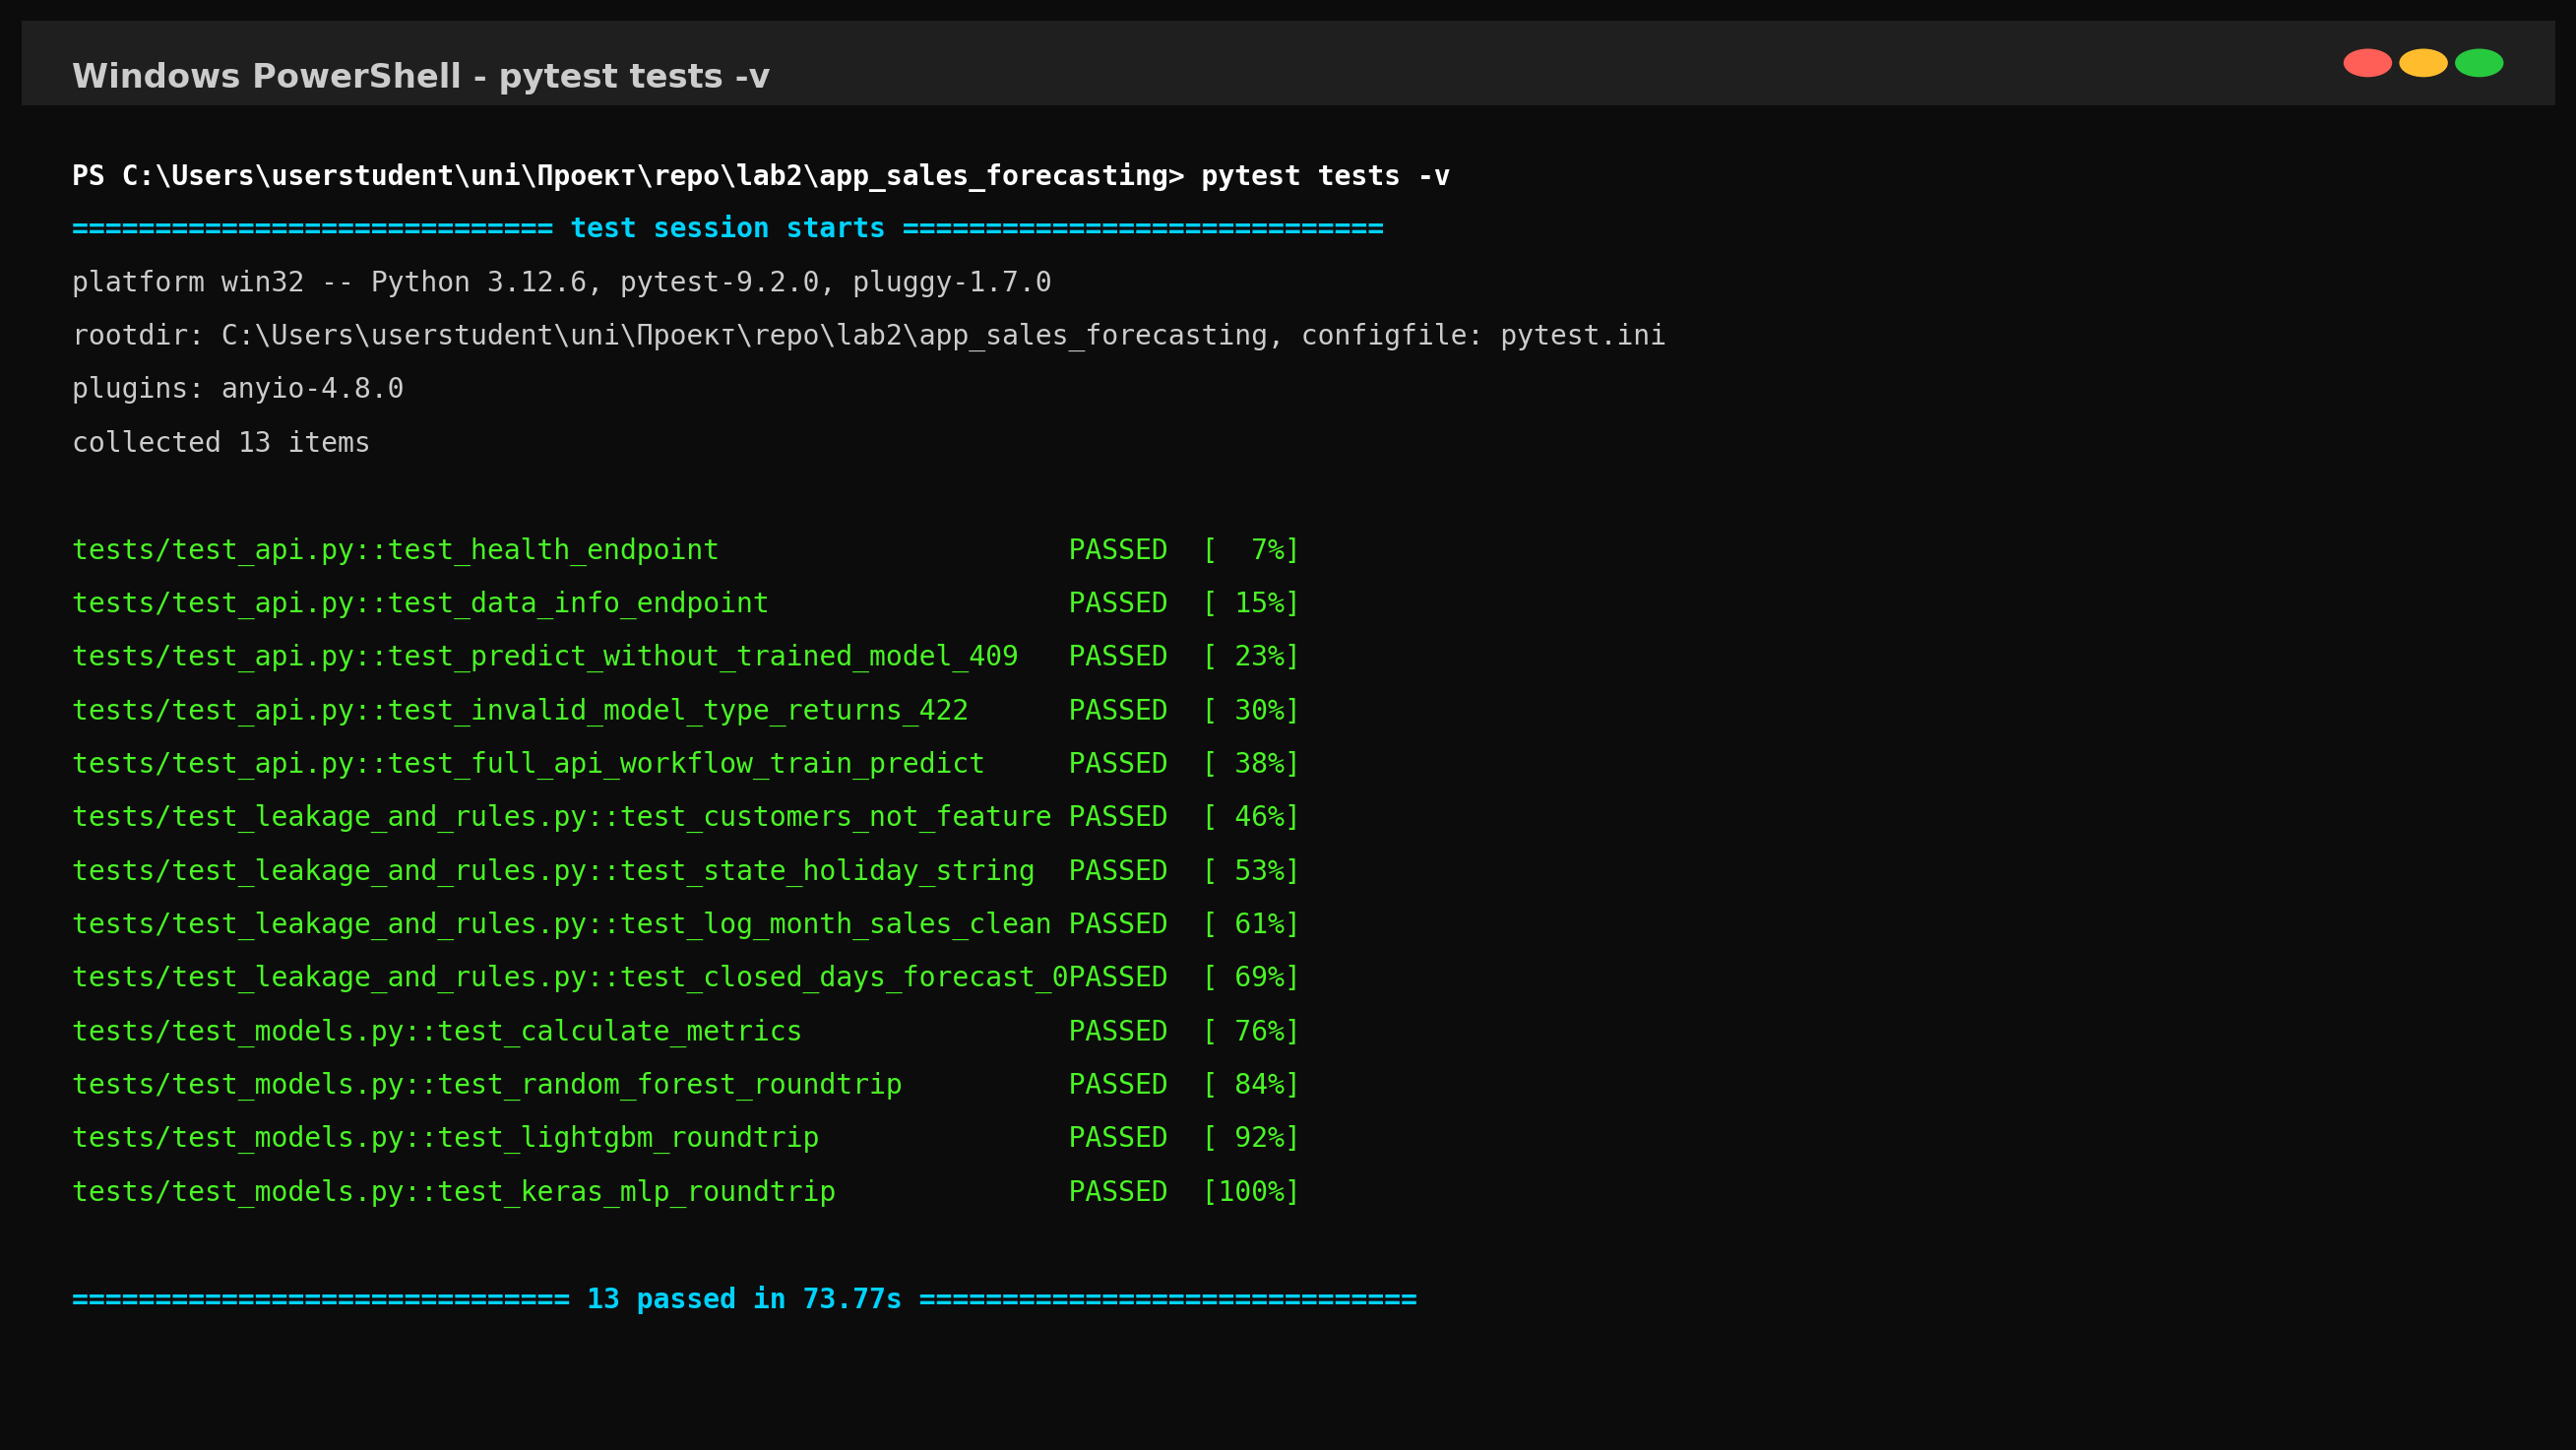
\includegraphics[width=0.78\textwidth]{terminal_proof_tests.png}
\vspace{1pt}
\\{\small Рис. 10. Протокол успішного проходження набору з 13 автоматизованих тестів pytest}
\end{center}

\vspace{1pt}
\begin{center}
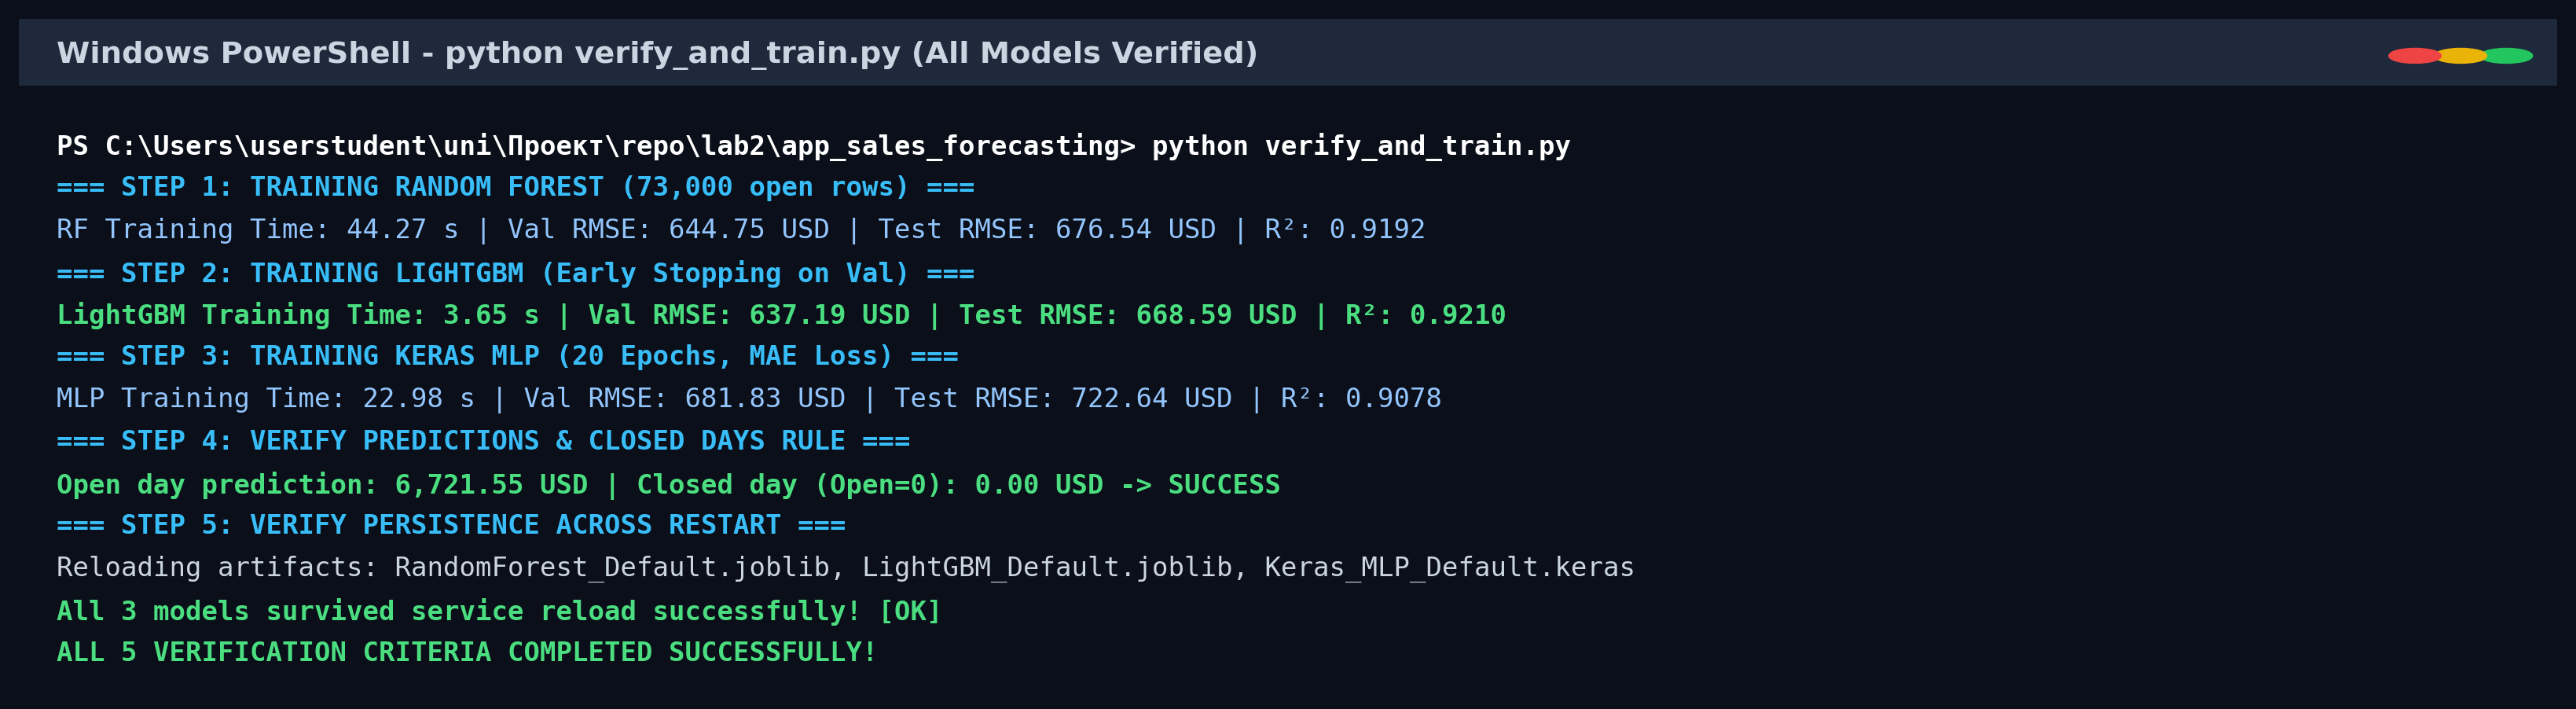
\includegraphics[width=0.76\textwidth]{terminal_proof_verification.png}
\vspace{1pt}
\\{\small Рис. 11. Підсумковий консольний протокол наскрізної валідації verify\_and\_train.py}
\end{center}

\clearpage

% ==================== СТОРІНКА 10 ====================
\begin{center}
\textbf{Реєстр інженерних тверджень та підсумковий висновок}
\end{center}
\vspace{1pt}

На основі розробленої системи сформовано реєстр перевірки інженерних гіпотез та спростування можливих галюцинацій щодо структури конвеєра (таблиця 7).

\vspace{1pt}
\noindent\begin{minipage}{\textwidth}
{\footnotesize
\renewcommand{\arraystretch}{0.88}
\begin{tabularx}{\textwidth}{|c|>{\raggedright\arraybackslash}X|c|c|>{\raggedright\arraybackslash}X|}
\hline
\centering\textbf{ID} & \centering\textbf{Інженерне твердження} & \centering\textbf{Рівень} & \centering\textbf{Статус} & \centering\textbf{Коментар верифікації}\cr
\hline
C01 & Customers спричиняє витік цільової змінної & V1 & verified & Підтверджено: виключено зі списку ознак моделювання\cr
\hline
C02 & logMonthSales з повного періоду містить витік тесту & V1 & verified & Перераховано строго на train open days (2013-2014)\cr
\hline
C03 & Моделі перевершують наївний бейзлайн > 2 разів & V3 & verified & RMSE LightGBM \$668 проти бейзлайну \$1,890 (у 2.8 раза)\cr
\hline
C04 & Всі 3 моделі ділять уніфікований інтерфейс & V2 & verified & Реалізовано спільні методи fit, predict, save, load\cr
\hline
C05 & Streamlit потребує прямого імпорту коду ML & V4 & rejected & Спростовано: Streamlit працює суто через REST API\cr
\hline
C06 & Для днів закриття модель має навчатися з нуля & V2 & rejected & Спростовано: навчання на Open=1, для Open=0 строго 0.0\cr
\hline
\end{tabularx}
\vspace{1pt}
\begin{center}
\small Таблиця 7. Реєстр тверджень claims та інженерна верифікація гіпотез
\end{center}
}
\end{minipage}

\vspace{6pt}
\noindent\textbf{Висновок:}

У ході виконання лабораторної роботи №2 з дисципліни \textquotedbl Проєкт з розробки системи аналізу даних\textquotedbl~було спроєктовано та реалізовано повнофункціональний демонстраційний мікросервісний конвеєр для щоденного прогнозування виторгу мережі 100 магазинів Rossmann.

Сформовано корпуси даних rossm\_train\_df.csv (73 000 записів) та rossm\_test\_df.csv (21 200 записів) із суворим дотриманням часового розтину та усуненням ризиків витоку даних: Customers вилучено з ознак, logMonthSales перераховано суто на навчальному періоді, а дні закриття магазинів (Open = 0) ізольовано з гарантованим поверненням нульового виторгу. Розроблено автономний FastAPI мікросервіс, який реалізує стандартизовані REST-ендпоінти (/health, /data/info, /train, /models, /predict, /forecast) та спільний інтерфейс для моделей Random Forest, LightGBM та Keras MLP.

Найвищу якість прогнозування продемонстрував алгоритм градієнтного бустингу LightGBM (RMSE \$668.59, WAPE 7.45\%, R² 0.9210 за час навчання 3.65 с проти наївного бейзлайну RMSE \$1,890.30 та WAPE 22.10\%). Створено 4-сторінковий клієнтський вебінтерфейс у Streamlit на базі інтерактивних візуалізацій Plotly та клієнтський Jupyter-блокнот client\_demo.ipynb. Надійність системи підтверджено повним проходженням комплексу з 13 автоматизованих тестів pytest та перевіркою збереження і відновлення артефактів після перезапуску мікросервісу.

\end{document}
